\chapter{\emph{In silico prediction of structure and function for a large family of transmembrane proteins that includes human Tmem41b}}

\section{Introduction}
Recent strides in computational structural biology have opened up an opportunity to understand previously uncharacterised proteins.  The under-representation of transmembrane proteins in the Protein Data Bank highlights the need to apply new and advanced bioinformatics methods to shed light on their structure and function. 

Membrane proteins can be grouped according to their interaction with various cell membranes: integral membrane proteins (IMPs) are permanently anchored whereas peripheral membrane proteins transiently adhere to cell membranes. IMPs that span the membrane are known as transmembrane proteins (TMEMs) as opposed to integral monotopic membrane proteins that adhere to one side of the membrane \cite{Fowler2006}. Membrane proteins also include various lipid-modified proteins \cite{Resh2016}.

Autophagy-related proteins (Atg) are responsible for the formation of autophagosomes that traffic unwanted intracellular components to the lysosomes for degradation.  Atg9 (Chapter 4) is the only established transmembrane Atg \cite{guardia2020structure}, however, there is a growing body of evidence that two proteins belonging to the Pfam PF09335 family may also be transmembrane Atgs; Tmem41b and Vmp1 \cite{Morita2019}. 

In this chapter, the Pfam PF09335 family is linked to the PF06695 family and a conveniently small archaeal sequence was identified. Subsequently, utilising state of the art methods, structural predictions for not only the archaeal sequence but also for two prominent members of the Pfam family PF09335 (Tmem41b and YqjA) were made. In order to carry out these predictions, data derived from sequence, evolutionary covariance and ab initio modelling was exploited. The result of the modelling indicated that both PF09335 homologues (DedA proteins) and PF06995 homologues contain re-entrant loops (stretches of protein that enter the bilayer but exit on the same side of the membrane).  Additionally, the predictions also anticipate that the re-entrant loops form part of a pseudo-inverted repeat topology. The predicted presence of both of these structural features strongly suggests that DedA proteins are secondary active transporters for an uncharacterised substrate.


\section{DedA Proteins}
The family Tmem41 has two human representatives, namely Tmem41a and Tmem41b; both share the PF09335 ('SNARE{\_}ASSOC'/ ‘VTT‘/’Tvp38’/’DedA’) Pfam \cite{El-Gebali2019} domain. The profile of Tmem41b has recently risen due to experimental evidence pointing to its involvement in macroautophagy regulation (making it a possible Atg protein, i.e. an autophagy related protein) and lipid mobilisation \cite{Moretti2018}. Other studies identify Tmem41b to be involved in motor circuit function, with TMEM41B-knockout \emph{Drosophila melanogaster} showing neuromuscular junction defects and aberrant motor neuron development in SMN1 knockout zebrafish \cite{Lotti2012}. Also, it has been reported that in TMEM41B-knockout HeLa cells there is an inhibition of Zika virus replication \cite{Scaturro2018}. Tmem41b has also been identified as a host cell factor for SARS-CoV-2 \cite{Schneider2020}. Tmem41b is the only common host cell factor identified for flaviviruses and coronaviruses and is the only autophagy-related protein identified as a viral host factor \cite{Hoffmann2021}.\\
Additionally, Tmem41b has been shown to be essential for mouse embryonic development: homozygous knockout mice embryos suffer early termination of their development after 7–8 weeks \cite{VanAlstyne2018}. Tmem41b is a structurally uncharacterised 291-residue protein found in the endoplasmic reticulum (ER) localising at the mitochondria-associated ER membranes \cite{Moretti2018}. Disruption of the PF09335 domain by various residue substitutions \cite{Tabara2019} or its removal \cite{Moretti2018} results in inhibition of autophagosome formation and impaired lipid mobilisation in human embryonic kidney (HEK) cells.\\
Tmem41b homologues, hereafter referred to as DedA proteins \cite{Morita2019}, are present in all domains of life \cite{Keller2013}. The Pfam PF09335 domain was first identified in the \emph{Saccharomyces cerevisiae} protein Tvp38 \cite{Inadome2007}, and the authors concluded that Tvp38 associates with SNARE proteins (SNAP REceptor).  SNARE proteins are responsible for the fusion of vesicles with a target membrane.  Specifically, Tvp38 was shown to associate with t-SNARE sub-types in Tlg2-containing compartments, suggesting a role in membrane transport. Investigations into the bacterial and archaeal prevalence of these proteins showed that 90\% of bacterial species and 70\% of archaeal species encode proteins with the PF09335 domain \cite{Doerrler2013}. Bacterial and archaeal PF09335-containing proteins are collectively known as the DedA family \cite{Doerrler2013,nonet1987hist}. Detailed studies of the \emph{Escherichia coli} DedA proteins have indicated that there are eight E. \textit{coli} representatives of the DedA family (YqjA, YghB, YabI, YohD, DedA, YdjX, YdjZ, and YqaA) with overlapping functions \cite{Doerrler2013,Keller2013}, with YdjX and YdjZ being the most closely related to human Tmem41b in terms of sequence similarity \cite{Doerrler2013}. Phenotypically, DedA knock-out \emph{E. coli} cells display increased temperature sensitivity, cell division defects, activation envelope stress pathways, compromised proton motive force, sensitivity to alkaline pH and increased antibiotic susceptibility \cite{Doerrler2013}\cite{Keller2014}. As \emph{E. coli} expresses multiple DedA homologues, lethal effects are not observed as long as at least one DedA is expressed \cite{Keller2014}\cite{Thompkins2008}. \emph{Borrelia burgdorferi} contains only one DedA protein in its genome and knockout cells display the same phenotype as the \emph{E. coli} knockout strains.  The \emph{B. burgdorferi} homologue is indeed essential \cite{Feng2010}. Interestingly, \emph{E. coli} knockout cells can be rescued with the B. burgdorferi homologue that shows only 19\% sequence identity with YqjA. The functions of DedA have also been studied in the pathogen \emph{Burkholderia thailandensis} where one family member was found to be required for resistance to polymyxin \cite{Panta2019}.

\section{Specific Methods}
This PhD coincided with a rapid development in the field of ab initio structure prediction.  The most advanced methods at the time were always utilised and as new methods and model databases were released these were employed to gather additional structural information as well as to validate previous modelling attempts. 

\subsection{Model building: trRosetta}
In order to test whether the modelling software could accurately capture the re-entrant loop-helix structural motif, a model representing the crystal structure of 6cb2 was constructed using both trRosetta and DMPfold \cite{Greener2019}. The crystal of 6cb2 is comparable in terms of size (293 residues) and has the common structural features (inverted repeat with two re-entrant/TMhelix structures) to the Tmem41b and its homologous proteins.  The output structure was structurally aligned against the crystal structure using DALI (server) and a gave Z-score of 35 for the trRosetta with 27.5 for the DMPfold equivalent. A significant Z-score indicates a higher level of structural similarity between two protein structures than would be expected by chance alone. In Dali, Z-scores greater than a certain threshold (typically around 2.0) are considered statistically significant, indicating a meaningful structural similarity between the compared proteins \cite{Holm2016}. Therefore, scores leave no doubt that the correct fold was modelled (figure \ref{fig:6cb2_super}) and therefore added to the confidence of any models constructed for PF09335 and PF06695 family members using trRosetta and DMPfold.  


\begin{figure}[th!]
    \centering
    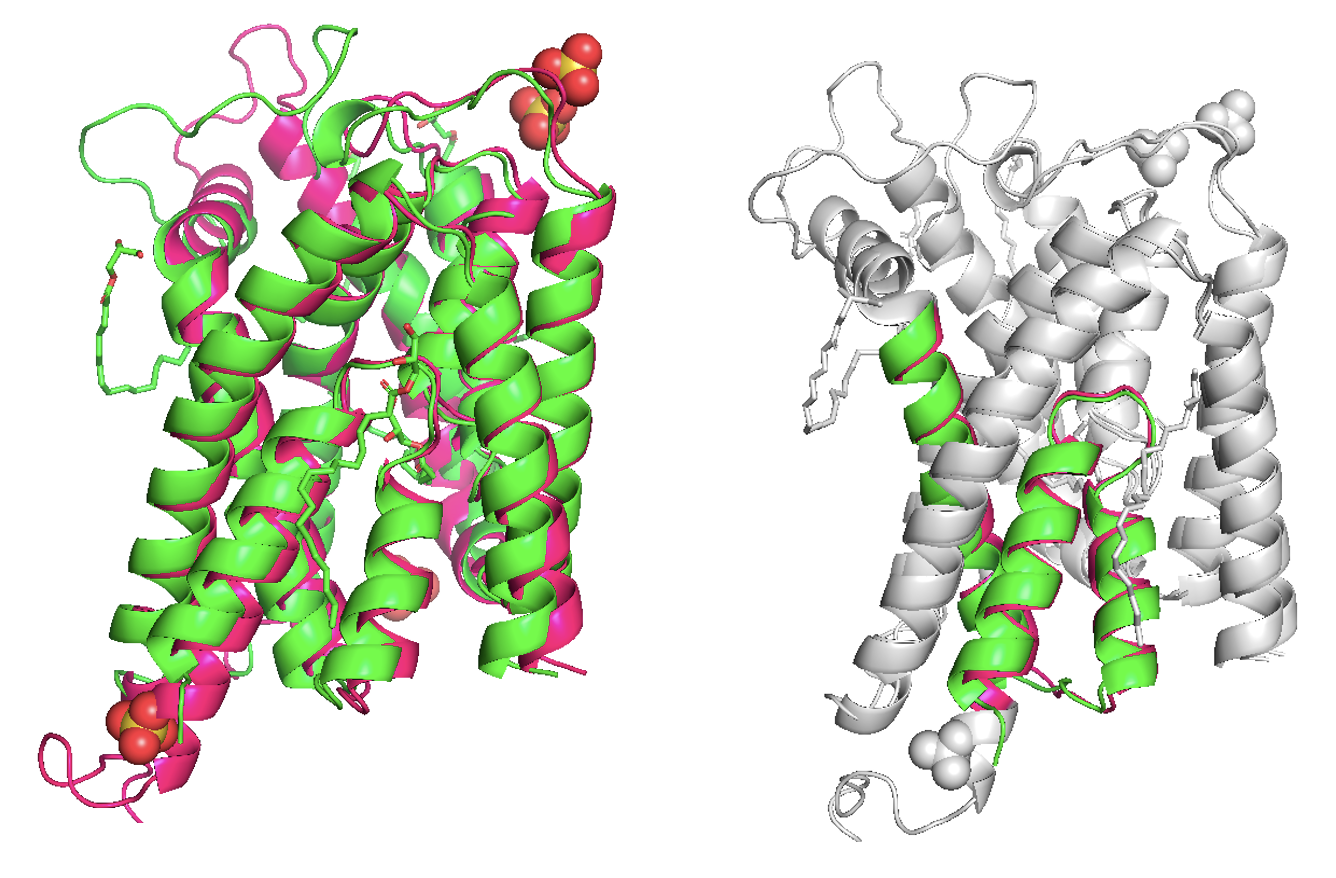
\includegraphics[width=\textwidth]{Results/6cb2_models.png}
    \caption{6cb2 Models}
    \label{fig:6cb2_super}
    \small
    The crystal structure in green and the trRosetta model in magenta.  The second image highlights the re-entrant structural motif feature that became prominent during the course of this investigation. 
\end{figure}


\subsection{Dataset for custom re-entrant sequence database}
A library of re-entrant loop sequences together with the putative re-entrant loop sequences from the Mt2055, Tmem41b and YqjA models were clustered to establish any visible relationships of the sequences. The library was built by obtaining a non-redundant set of 56 re-entrant helix sequences by first retrieving all 714 TM proteins that contain at least one re-entrant loop from the PDBTM \cite{Kozma2012} and removing redundancy with a 40\% identity threshold. The resulting 127 protein structures were split into their component chains, eliminating any chain lacking a re-entrant loop. The resulting set of 188 unique re-entrant loop sequences were then filtered removing any sequences of less than 10 residues and more than 20, thereby ensuring the collection of sequences conformed to the length of typical \cite{Yan2010} re-entrant loops. The remaining 56 sequences were clustered, supplemented by candidate re-entrant sequences from the proteins studied here. Clustering was performed using CLANS v1.0 \cite{Frickey2004} with the BLAST \cite{Altschul1997} results used to calculate strengths of similarity.

\subsection{Dataset for custom structural re-entrant database}
In addition to the construction of the re-entrant sequence database a structural database was also built for the re-entrant loops in the PDBTM. A library of re-entrant loop pdb structures together with the putative re-entrant loop structures from the Mt2055, Tmem41b and YqjA protein models were clustered on their structural similarity. The library was built by obtaining a non-redundant (removing redundancy with a 40\% sequence identity threshold) set of 125 chains from the PDBTM \cite{Kozma2012} that contain at least one re-entrant loop. 40\% sequence identity threshold is considered to be a reasonably stringent criterion for redundancy removal. It ensures that the retained homologues have a significant level of similarity with the query sequence, indicating a high likelihood of shared evolutionary ancestry and potential functional conservation. As this investigation focuses on re-entrant loops that are immediately preceded by a TM helix that is packed against the loop, all re-entrant loops (boundaries defined by PDBTM) in addition to the preceding 30 residues were extracted. The resulting 193 library entries, supplemented with the re-entrant loop features (defined by the OMP server \cite{Lomize2012} and accompanied by the preceding 30 residues) from the ab initio modelling underwent an all-against-all structural alignment using a local installation of Dali v4.0 \cite{Holm2016}. The Z-scores for these alignments were then used for clustering with CLANS v1.0 \cite{Frickey2004} with a Z-score of 4.5 used as the cut-off threshold.

\section{Sequence Analysis}
HHpred \cite{Zimmermann2018} was used to screen a selection of DedA proteins against the Pfam database \cite{El-Gebali2019}. Hits were observed in the same region against both PF09335 and the Pfam domain PF06695 (‘Sm{\_}multidrug{\_}ex’) which is strongly indicative of homology: a probability of 99.4\% with an E-value of 9E-17 for the PF09335 hit and 98.3\% and 2E-10 respectively for PF06695. An HHpred search against the Pfam database using a member of PF06695 - the short archaeal sequence Mt2055 (UniProt code W9DY28) \cite{Apweiler2004} - returned similar results (Table \ref{table:hhpred} ). Figure \ref{fig:msa} shows the MSA for the same sequences along with the relative positions of the two Pfam domains under investigation.  The Mt2055 sequence originates from the unpublished draft genome of the archaebacterium Methanolobus tindarius DSM 2278.  For many of the subsequent analyses, the shorter archaeal sequence was used initially but the clear homology among this set of proteins means that inferences can be drawn across the group.

\begin{table}[]
\caption{HHpred results for Tmem41b and homologues demonstrate homology between Pfam families PF09335 and PF06695.}
\centering
\resizebox{\columnwidth}{!}{%
\begin{tabular}{llllllll}
\rowcolor[HTML]{BDCCD4} 
\multicolumn{2}{l}{\cellcolor[HTML]{BDCCD4}{\color[HTML]{666666} \textbf{}}}                                                  & \multicolumn{2}{l}{\cellcolor[HTML]{BDCCD4}{\color[HTML]{666666} \textbf{}}}                                                    & \multicolumn{2}{l}{\cellcolor[HTML]{BDCCD4}{\color[HTML]{666666} \textbf{\begin{tabular}[c]{@{}l@{}}PF09335\\ 'SNARE\_ASSOC'/ \\ ‘VTT ‘/’Tvp38’\end{tabular}}}} & \multicolumn{2}{l}{\cellcolor[HTML]{BDCCD4}{\color[HTML]{666666} \textbf{\begin{tabular}[c]{@{}l@{}}PF06695\\ ‘Sm\_multidrug\_ex’\end{tabular}}}} \\
\rowcolor[HTML]{BDCCD4} 
{\color[HTML]{666666} \textbf{}} & {\color[HTML]{666666} \textbf{Species}}                                                    & {\color[HTML]{666666} \textbf{\begin{tabular}[c]{@{}l@{}}UniProt\\ Code\end{tabular}}} & {\color[HTML]{666666} \textbf{Length}} & {\color[HTML]{666666} \textbf{Probability}}                                          & {\color[HTML]{666666} \textbf{E-Value}}                                         & {\color[HTML]{666666} \textbf{Probability}}                                   & {\color[HTML]{666666} \textbf{E-Value}}                                  \\
\rowcolor[HTML]{FFFFFF} 
{\color[HTML]{666666} Tmem41b}   & {\color[HTML]{666666} \begin{tabular}[c]{@{}l@{}}Homo \\ sapiens\end{tabular}}             & {\color[HTML]{666666} Q5BJD5}                                                          & {\color[HTML]{666666} 291}             & {\color[HTML]{666666} 99.4}                                                   & {\color[HTML]{666666} 9E-17}                                                    & {\color[HTML]{666666} 98.3}                                            & {\color[HTML]{666666} 2E-10}                                             \\
\rowcolor[HTML]{E5EBEF} 
{\color[HTML]{666666} Ydjx}      & {\color[HTML]{666666} \begin{tabular}[c]{@{}l@{}}Escherichia \\ coli\end{tabular}}         & {\color[HTML]{666666} P76219}                                                          & {\color[HTML]{666666} 236}             & {\color[HTML]{666666} 99.6}                                                   & {\color[HTML]{666666} 2.1E-17}                                                  & {\color[HTML]{666666} 99.1}                                            & {\color[HTML]{666666} 9.9E-13}                                           \\
\rowcolor[HTML]{FFFFFF} 
{\color[HTML]{666666} Ydjz}      & {\color[HTML]{666666} \begin{tabular}[c]{@{}l@{}}Escherichia \\ coli\end{tabular}}         & {\color[HTML]{666666} P76221}                                                          & {\color[HTML]{666666} 235}             & {\color[HTML]{666666} 99.6}                                                   & {\color[HTML]{666666} 1.1E-17}                                                  & {\color[HTML]{666666} 99.0}                                            & {\color[HTML]{666666} 4.5E-16}                                           \\
\rowcolor[HTML]{E5EBEF} 
{\color[HTML]{666666} Yqja}      & {\color[HTML]{666666} \begin{tabular}[c]{@{}l@{}}Escherichia \\ coli\end{tabular}}         & {\color[HTML]{666666} P0AA63}                                                          & {\color[HTML]{666666} 220}             & {\color[HTML]{666666} 99.62}                                                  & {\color[HTML]{666666} 5.6E-15}                                                  & {\color[HTML]{666666} 99.41}                                           & {\color[HTML]{666666} 1.3E-12}                                           \\
\rowcolor[HTML]{FFFFFF} 
{\color[HTML]{666666} Tvp38}     & {\color[HTML]{666666} \begin{tabular}[c]{@{}l@{}}Saccharomyces \\ cerevisiae\end{tabular}} & {\color[HTML]{666666} P36164}                                                          & {\color[HTML]{666666} 337}             & {\color[HTML]{666666} 99.4}                                                   & {\color[HTML]{666666} 7.9E-15}                                                  & {\color[HTML]{666666} 98.7}                                            & {\color[HTML]{666666} 2.7E-10}                                           \\
\rowcolor[HTML]{E5EBEF} 
{\color[HTML]{666666} Mt2055}    & {\color[HTML]{666666} \begin{tabular}[c]{@{}l@{}}Methanolobus \\ tindarius\end{tabular}}   & {\color[HTML]{666666} W9DY28}                                                          & {\color[HTML]{666666} 168}             & {\color[HTML]{666666} 99.0}                                                   & {\color[HTML]{666666} 2.4E-10}                                                  & {\color[HTML]{666666} 99.8}                                            & {\color[HTML]{666666} 1.8E-20}                                          
\end{tabular}
}
\label{table:hhpred}
\end{table}

\begin{figure}[th!]
    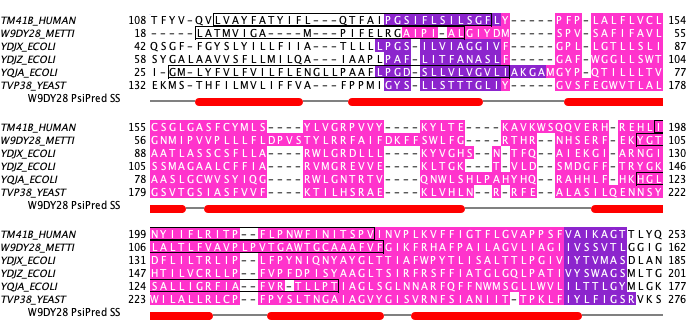
\includegraphics[width=\textwidth]{Results/fig1.png}
    \caption{MSA for query protein selection listed in table \ref{table:hhpred}.}
    \label{fig:msa}
    \small
    Magenta highlights the regions matched by HHpred to the PF06695 Pfam domain while purple is used for additional residues included in the PF09335 Pfam domain matches. The black boxed regions represent the locations of the putative re-entrant loops as identified by the modeling of the respective proteins. The secondary structure for the archaeal W9DY29 sequence (Mt2055) is also depicted with the relative positions of alpha helices shown as red blocks.
\end{figure}

There are no known experimental protein structures representing PF09335 or PF06695, but both Gremlin and DMPfold have constructed ab initio models for these Pfam domains and have made them available in repositories \cite{Greener2019, Ovchinnikov2017}.

Analysis of the HHpred results obtained for the archaeal protein Mt2055 revealed the presence of additional hits for both PF06695 and PF09335 Pfam domains, in which the C-terminal half of the domains aligned with the N-terminal half of the Archaea protein. For example, residues 1-69 of the archaeal protein aligned with residues 52-117 of the Pfam PF09335 profile with a probability of 74.15\%.

Interestingly, contact density analysis \cite{Rigden2002}\cite{Sadowski2013} supported the existence of a domain boundary around residue 60, in broad agreement with the HHpred results (Figure \ref{fig:w9_dom_anal}). Both the HHpred and contact density results therefore pointed to a specific domain structure being present.

\begin{figure}[th!]
    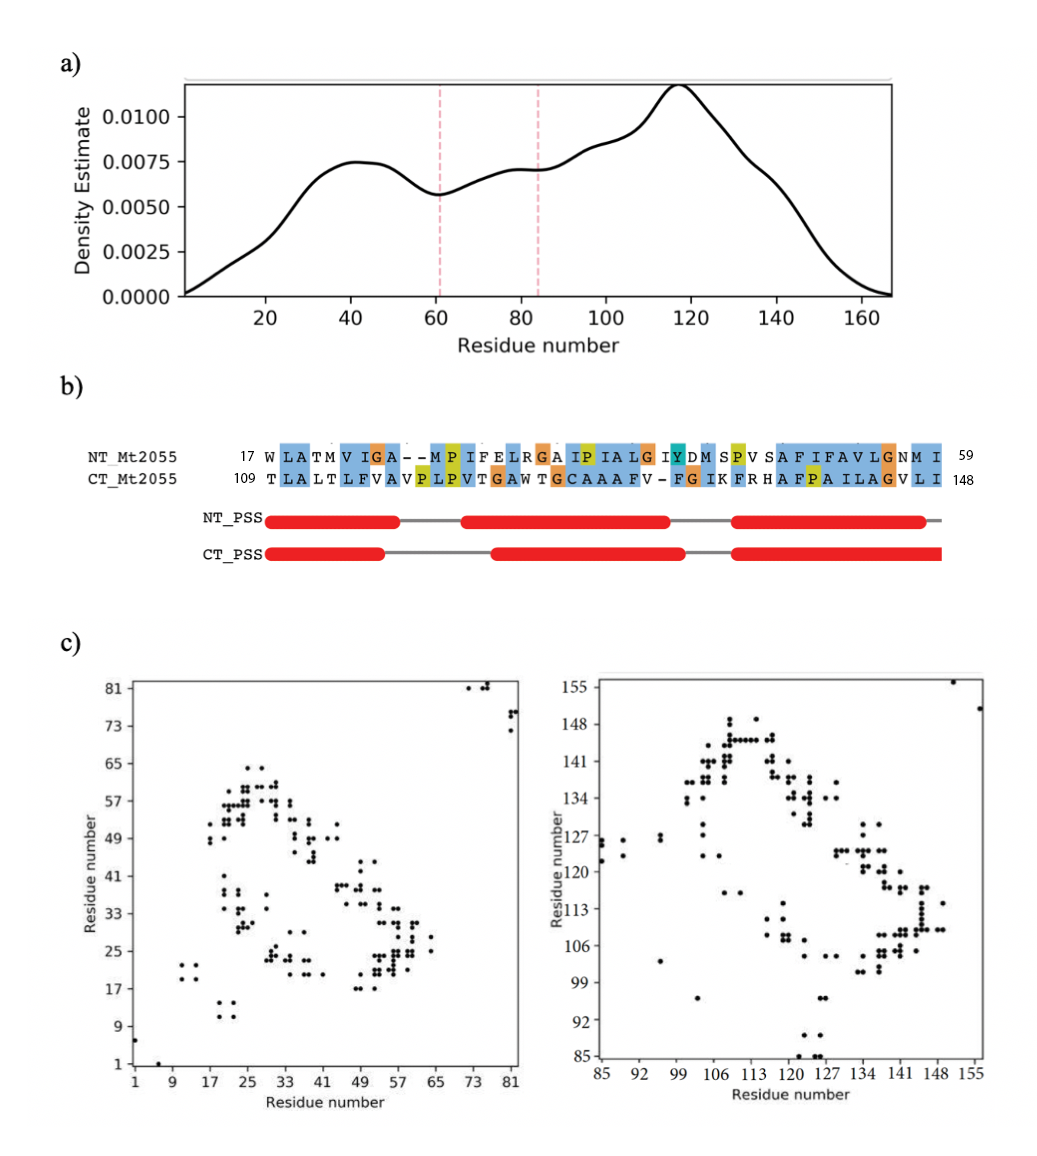
\includegraphics[width=\textwidth]{Results/fig2.png}
    \caption{Mt2055 domain analysis. }
    \label{fig:w9_dom_anal}
    \small
    (a) Contact density profile constructed by ConKit \cite{Simkovic2017} utilising DeepMetaPSICOV contact prediction. Solid black line represents contact density and dotted red lines mark density minima corresponding to possible domain boundaries. (b) HHalign alignments for the N-terminal and C-terminal Mt2055 halves, formatted using Jalview \cite{Waterhouse2009} and coloured according to the ClustalX \cite{jeanmougin1998multiple} scheme. Red bars represent helical secondary structure. (c) Maps of predicted contacts generated by DeepMetaPSICOV \cite{Kandathil2019} and plotted using ConKit \cite{conkit2017}; left is N-terminal half (residues 1-84) and right is C-terminal half (residues 85-168). Black points represent predicted intramolecular contacts.
\end{figure}

When the Mt2055 sequence was split at residue 60-61, the resulting N-terminal region of 60 residues and the C-terminal section of 79 residues could be aligned using HHalign \cite{Soding2005} with a 78\% probability and an E-value of 1.9E-3. Examination of the map of predicted contacts for Mt2055 reveals features that are present in both the N- and C-terminal halves of the protein (Figure \ref{fig:w9_dom_anal}c). Taken together, these data strongly support the existence of a tandem repeat within the Mt2055 protein and hence across the PF06695 and PF09335 protein families.\\
Interestingly, an equivalent sequence analysis with HHpred of other PF09335 homologues including Tmem41b itself does not reveal a repeat. However, inspection of their corresponding predicted contact maps does reveal features repeated when N- and C-halves of the protein are compared (Figure \ref{fig:tm_c_map}). Apparently, evolutionary divergence has removed all trace of the repeat sequence signal in bacterial and eukaryotic proteins, although the feature remains visible by evolutionary covariance analysis.\\

In order to assess the composition of the repeat identified, transmembrane helical topology predictions were carried out but gave inconsistent results for most proteins: only for the archaeal protein Mt2055 did all methods agree that four transmembrane helices were predicted to be present in the whole protein, two in each of the repeats (Table \ref{table:tm_pred}).

\begin{table}
\caption{Predicted number of TM regions for PF09335/PF06695 homologs}
\resizebox{\columnwidth}{!}{%
\centering
\begin{tabular}{lccccccc}
\rowcolor[rgb]{0.753,0.753,0.753} ~         & \multicolumn{1}{l}{TOPCONS} & \multicolumn{1}{l}{OCTOPUS} & \multicolumn{1}{l}{PHILIUS} & \multicolumn{1}{l}{POLYPHOBIUS} & \multicolumn{1}{l}{SCAMPI} & \multicolumn{1}{l}{SPOCTOPUS} & \multicolumn{1}{l}{TMHMM}  \\
{\cellcolor[rgb]{0.753,0.753,0.753}}Mt2055  & 4                           & 4                           & 4                           & 4                               & 4                          & 4                             & 4                          \\
{\cellcolor[rgb]{0.753,0.753,0.753}}Tmem41b & 6                           & 6                           & 6                           & 7                               & 6                          & 5                             & 6                          \\
{\cellcolor[rgb]{0.753,0.753,0.753}}Ydjx    & 7                           & 7                           & 5                           & 6                               & 6                          & 7                             & 5                          \\
{\cellcolor[rgb]{0.753,0.753,0.753}}Ydjz    & 6                           & 7                           & 6                           & 6                               & 6                          & 6                             & 5                          \\
{\cellcolor[rgb]{0.753,0.753,0.753}}Tvp38   & 5                           & 7                           & 5                           & 7                               & 6                          & 6                             & 5                         
\end{tabular}
}
\label{table:tm_pred}
\end{table}

\begin{figure}[th!]
    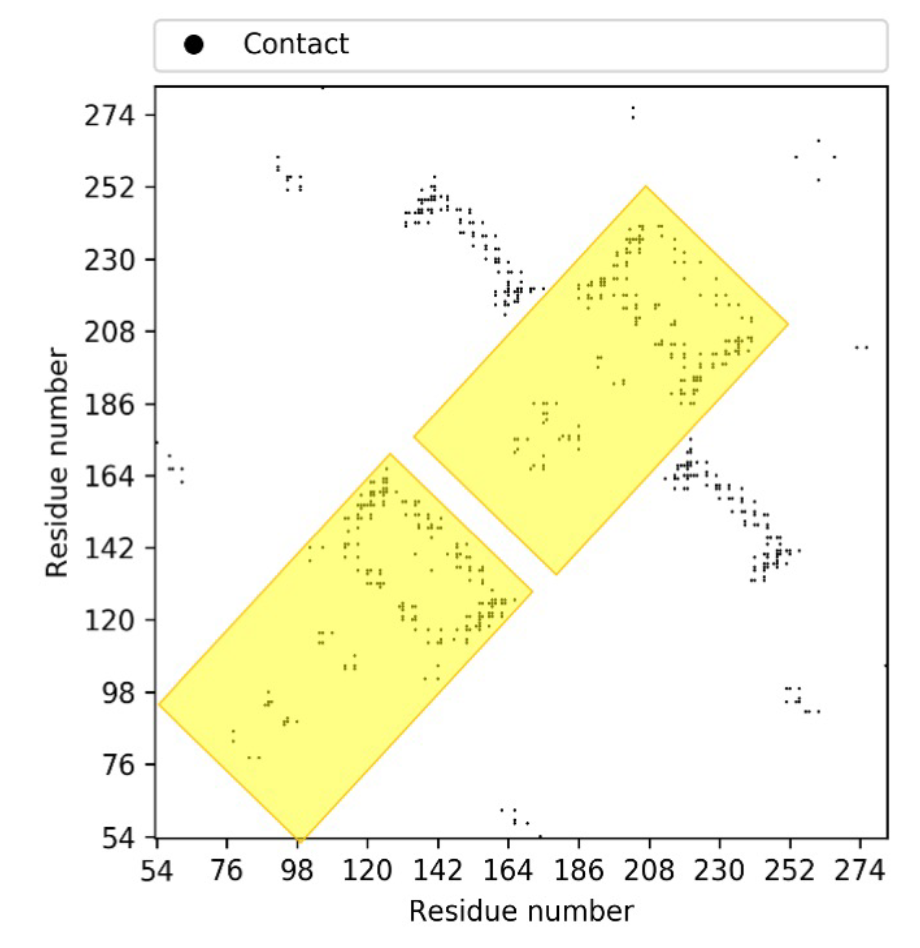
\includegraphics[width=\textwidth]{Results/fig3.png}
    \caption{Tmem41b Contact map constructed using DeepMetaPSICOV and plotted using Conkit.}
    \label{fig:tm_c_map}
    \small
    The highlighted areas represent repeat units that have been revealed through evolutionary covariance analysis.
\end{figure}

Several authors have deposited structures of uncharacterised Pfam families in databases \cite{El-Gebali2019}; however, Pfam domain boundaries for PF09335/PF06695, which define the limits of these previous modelling exercises, do not reflect the conserved structural domain that we predict. Given the fact that the available ab initio models were inconsistent with the transmembrane helix topology, secondary structure and contact predictions, new models of Mt2055 as well as Tmem41b and YqjA were built. 

\section{Initial Modelling}
Initial modelling of DedA proteins centered around constructing DeepContact \cite{Liu2018} derived contact restrained Mt2055 models using Rosetta \emph{ab initio}.  The output models were visually of very poor quality and could not possibly be stable within a membrane.  Subsequently, in an effort to improve the quality of the contact information a metagenomics \cite{Ovchinnikov2017} sequence database was used to generate the predicted contacts.  The MapPred \cite{wu2020protein} server was used to trial the use of metagnomics; for Mt2055 the Neff of the MSA was raised to 2687 from the  1648 Uniprot-derived MSA; for Tmem41b the Neff of the MSA was raised to 8874 from the 2144 Uniprot derived MSA.  The success at raising the Neff values of the MSAs for the query proteins led to the construction of a custom metagenomics sequence database. JackHMMER \cite{Johnson2010} was used to generate the MSAs and ResPre \cite{Li} to make the contact predictions based on the metagenomics enhanced MSAs.  With the custom metagenomics database, for Mt2055 the Neff reached 7470 and for Tmem41b the Neff increased to 88573.  Figure \ref{fig:seq_coverage} shows how the increase in Neff translated to local sequence regions  with the use of series of sequence coverage plots generated using ConKit \cite{conkit2017}; for example for Tmem41b, even though the metagenomic improved the global Neff score dramatically, the MSA coverage profile does highlight the fact that the metegenomics has little impact on the first one hundred residues.

\begin{figure}[th!]
    \makebox[\textwidth]{\includegraphics[width=\paperwidth]{...}}
    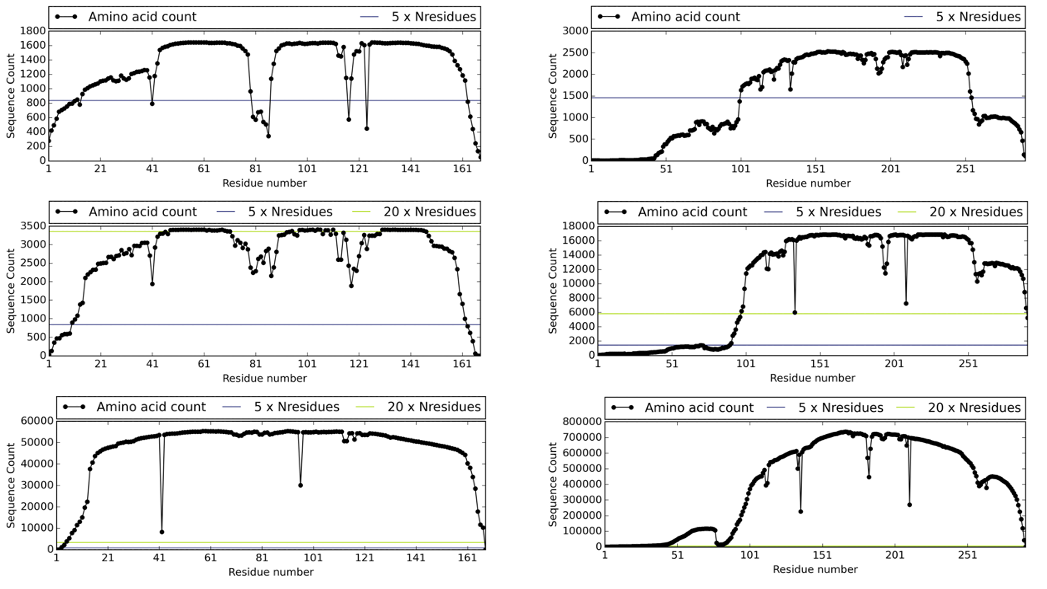
\includegraphics[width=\textwidth]{Results/meta_fig.png}
    \caption{MSA Sequence coverage profiles.}
    \label{fig:seq_coverage}
    \small
    Column 1: Mt2055, Column 2: Tmem41b, Row 1: Uniprot derived, Row 2: MapPred derived, Row 3: Custom metagenomics database derived.
\end{figure}

Again, even with the metagenomic enhanced contact predictions, the poor model quality could be visually identified (short transmembrane helices -less than 5 helical turns- that could not possibly span the lipid bi-layer) and quantitatively measured using a contact satisfaction profile plotted using ConKit (figure \ref{fig:precision}).  Running these models as well as the examples from the previous set against the PDB using Dali \cite{Holm2016} to identify possible stuructural homologues did not yield any significant results with the top Z-score being 3.5.

\begin{figure}[th!]
    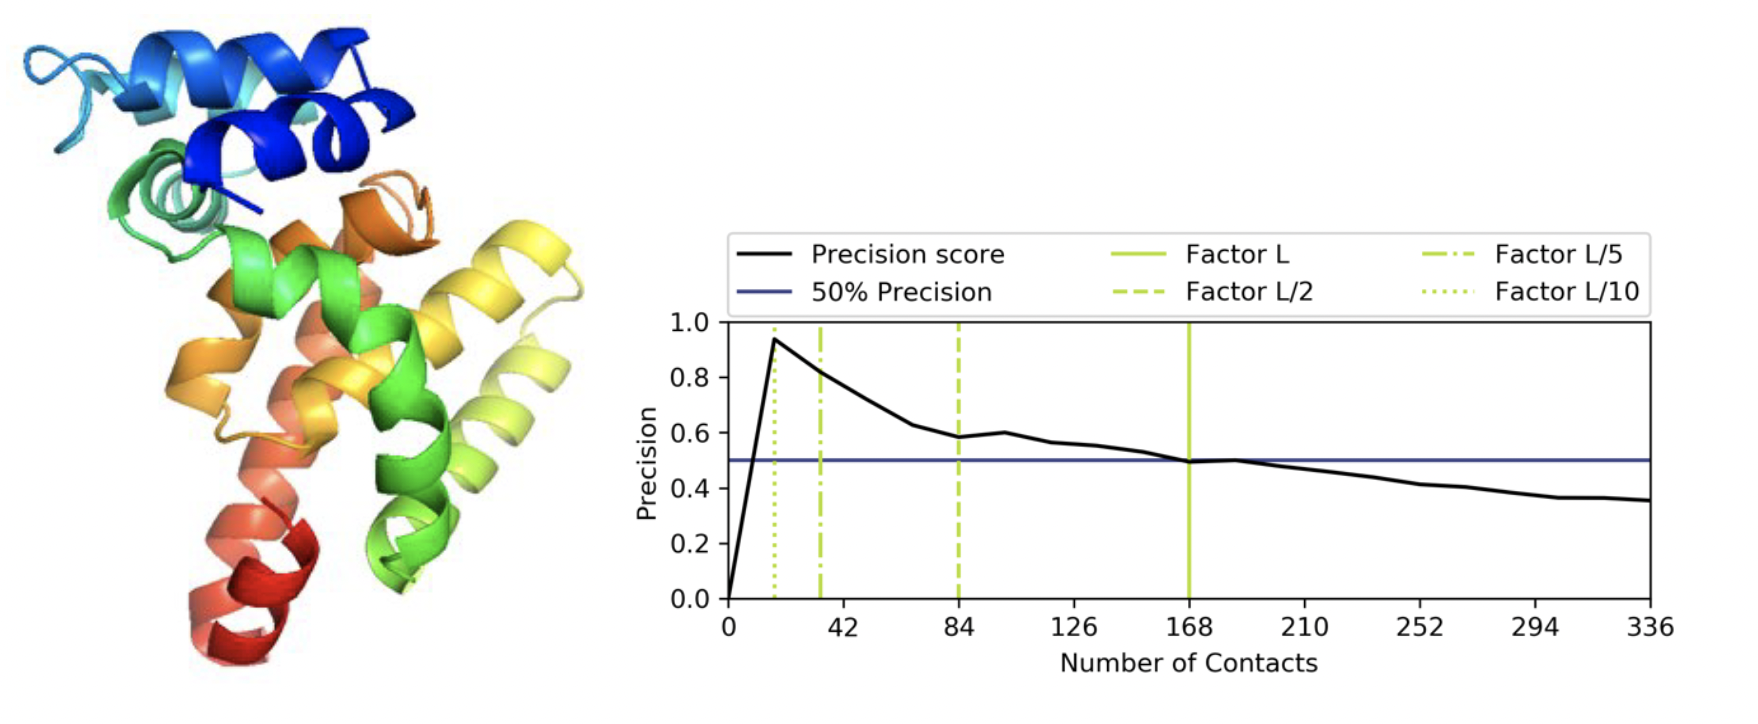
\includegraphics[width=\textwidth]{Results/meta_ros_model_fig.png}
    \caption{Rosetta Ab initio model with Precision Profile.}
    \label{fig:precision}
    \small
    Left: Mt2055 Rosetta ab initio model utilising restraints derived from Respre (Li et al.,
n.d.) and a metagenomic database for MSA construction; coloured with rainbow; blue C -terminal
to red N-terminal; right: precision profile depicting contact satisfaction at various contact cutoff values where L = sequence length (rounded down to the nearest whole number of contacts). The 50\% precision cut of is shown (blue line) as a visual marker. A minimum of 70\% contact satisfaction for the top L contacts would be suggestive of good quality models \cite{de2017comparing}..
\end{figure}

Building on the premise of utilising the contacts as restraints in the model making, it was decided to switch to the Rosetta Ab initio Membrane protocol \cite{alford2015integrated}.  This version of Rosetta \textit{ab initio}, in addition to the contact derived restraints, uses membrane topology predictions as further restraints and are more heavily weighted than the contact information.  TopCons \cite{Tsirigos2015} was used to generate the membrane topology predictions for the query proteins which were subsequently converted into the Rosetta Membrane compatible OCTOPUS \cite{Viklund2008} format.\\

One thousand models were constructed. The output models from the RosettaMembrane flavour were visually superior to the outputs from Rosetta ab initio;  these models possessed helices packed together in such a way that they could conceivably sit in a membrane bi-layer.  Screening the highest ranking model (centroid of the largest cluster determined by SPICKER \cite{Zhang2004}) against the PDB using DALI and filtering out globular proteins and all hits with a Z-score less than 5 resulted in a list of strong hits with Type VII ABC transporters (Table \ref{table:abc}) with the strongest hit against 5lilA (Figure \ref{fig:5lil_super}). \\

In an effort to identify a potentially stronger hit from the one thousand models, the set of models were processed into a local DALI database and 5lilA was used to query the library.  However, the same model with a Z-score of 8.8 was picked out.  Consequently a further ten thousand RosettaMembrane models were constructed and 5lil was screened against this new model set.  A model with a Z-score of 9.9 was identified.

\begin{table}
\caption{DALI PDB hits with top model from first round of RosettaMembrane modelling}
\resizebox{\columnwidth}{!}{%
\centering
\begin{tabular}{lllllll}
\rowcolor{cyan} Hit                  & Z-Score & RMSD & lali & Nres & \%ID & Hit Name                                           \\
\rowcolor[rgb]{0.137,1,0.769} 5lil-A & 8.8     & 3.8  & 131  & 615  & 12   & MACROLIDE EXPORT ATP-BINDING/PERMEASE PROTEIN MAC  \\
\rowcolor{cyan} 5lj6-A               & 8.3     & 5    & 132  & 600  & 8    & MACROLIDE EXPORT ATP-BINDING/PERMEASE PROTEIN MAC  \\
\rowcolor[rgb]{0.137,1,0.769} 5lj7-B & 8       & 4.9  & 132  & 599  & 8    & MACROLIDE EXPORT ATP-BINDING/PERMEASE PROTEIN MAC  \\
\rowcolor{cyan} 5lil-B               & 7.1     & 4.9  & 132  & 604  & 8    & MACROLIDE EXPORT ATP-BINDING/PERMEASE PROTEIN MAC  \\
\rowcolor[rgb]{0.137,1,0.769} 5mal-A & 7       & 3.9  & 104  & 234  & 14   & LIPASE;                                            \\
\rowcolor{cyan} 5lj7-A               & 6.7     & 4    & 125  & 592  & 11   & MACROLIDE EXPORT ATP-BINDING/PERMEASE PROTEIN MAC  \\
\rowcolor[rgb]{0.137,1,0.769} 5mal-B & 6.6     & 3.5  & 103  & 234  & 15   & LIPASE;                                            \\
\rowcolor{cyan} 5ws4-B               & 6.4     & 4    & 129  & 650  & 8    & MACROLIDE EXPORT ATP-BINDING/PERMEASE PROTEIN MAC  \\
\rowcolor[rgb]{0.137,1,0.769} 6fpf-A & 6.3     & 3.9  & 125  & 257  & 6    & CHROMOSOME 16, WHOLE GENOME SHOTGUN SEQUENCE;      \\
\rowcolor{cyan} 5ws4-A               & 6.3     & 4    & 129  & 650  & 8    & MACROLIDE EXPORT ATP-BINDING/PERMEASE PROTEIN MAC  \\
\rowcolor[rgb]{0.137,1,0.769} 5gtm-B & 6.2     & 6.2  & 92   & 522  & 12   & INTERFERON-INDUCED GTP-BINDING PROTEIN MX1;        \\
\rowcolor{cyan} 5nil-J               & 6.1     & 4.2  & 131  & 629  & 13   & OUTER MEMBRANE PROTEIN TOLC;                       \\
\rowcolor[rgb]{0.137,1,0.769} 5nik-J & 6.1     & 4.2  & 131  & 629  & 13   & OUTER MEMBRANE PROTEIN TOLC;                       \\
\rowcolor{cyan} 5gko-B               & 6.1     & 3.8  & 126  & 650  & 8    & MACROLIDE EXPORT ATP-BINDING/PERMEASE PROTEIN MAC  \\
\rowcolor[rgb]{0.137,1,0.769} 5nik-K & 5.9     & 4.4  & 133  & 629  & 12   & OUTER MEMBRANE PROTEIN TOLC;                       \\
\rowcolor{cyan} 5nil-K               & 5.9     & 4.4  & 133  & 629  & 12   & OUTER MEMBRANE PROTEIN TOLC;                       \\
\rowcolor[rgb]{0.137,1,0.769} 5do7-C & 5.8     & 5.3  & 129  & 579  & 7    & ATP-BINDING CASSETTE SUB-FAMILY G MEMBER 5;       
\end{tabular}
}
\label{table:abc}
\end{table}

\begin{figure}[th!]
    \centering
    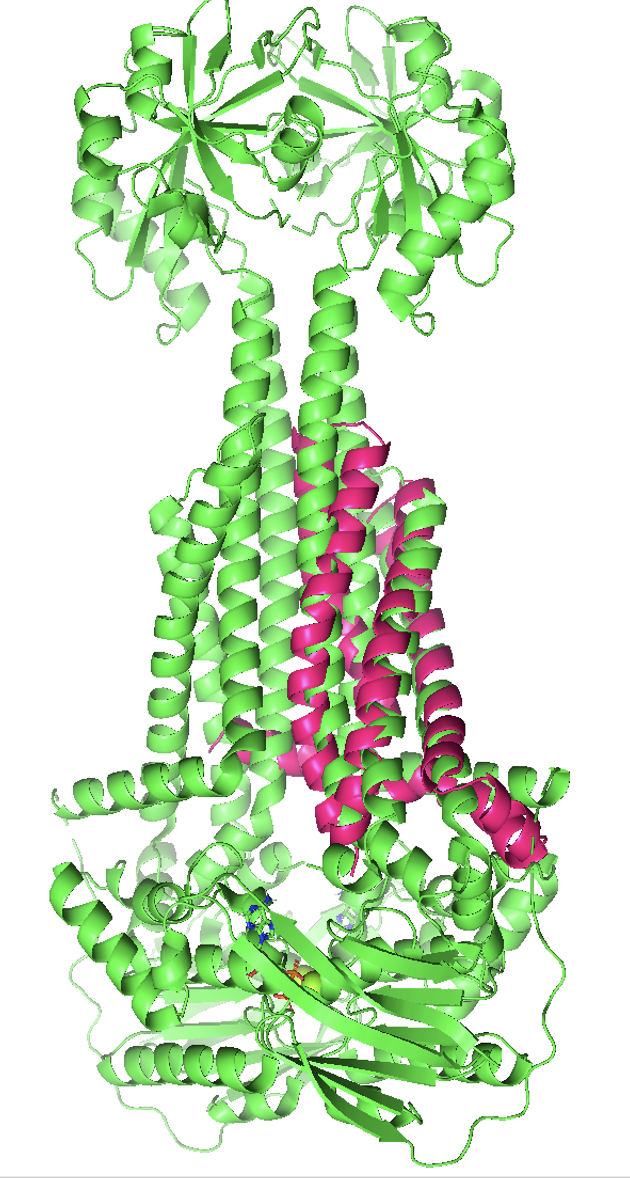
\includegraphics[width=50mm, scale =0.5]{Results/5lil_super_fig.png}
    \caption{Rosetta Membrane model structurally aligned with 5lilA.}
    \label{fig:5lil_super}
    \small
    Rosetta Ab initio Membrane model (magenta) structurally aligned with 5lil (green).
\end{figure}

Next the idea of refining the model based on use of contact restraints was experimented with; the contacts from the model with the highest alignment Z-score with 5lil were used as restraints to construct a further ten thousand new models.  The output models were again converted to a DALI database and 5lil was screened against the new library.  This additional refinement step did not produce models with any higher alignment scores with 5lil.  A comparison of the 5lil contact map and the model contact map \ref{fig:5lil_cmaps} clearly showed that they certainly shared the transmembrane helical topology.  Study of the structural alignment (figure \ref{fig:5lil_schem}) also confirmed this. Additionally, both the model and 5lil possessed an amphipathic helix, albeit in the opposite direction (although this would not have contributed to the DALI Z-score calculation as only the aligned regions are used for this calculation).\\

5lil was an interesting structural hit. The fold and topology of the MacB transmembrane and periplasmic domain is different from the six other ABC transporter superfamilies and has an independent evolutionary origin from other ABC transporters. 5lil has a four-transmembrane helix topology, periplasmic domain, and stalk.  5lil forms a pump with TolC,  this complex uses cytoplasmic ATP hydrolysis to move substrates from the periplasm to the outside of the cell. 5lil is not considered a transporter as the ATP hydrolysis is used to transmit a conformational changes from cytoplasmic side of the membrane to the periplasmic side; TolC is responsible for the movement of substrate from the periplasm to the outside of the cell. It is the transmembrane domain of 5lil that is responsible for this mechanotransmission \cite{pichoff2019roles}.

\begin{figure}[htb]
    \centering % <-- added
\begin{subfigure}{0.25\textwidth}
  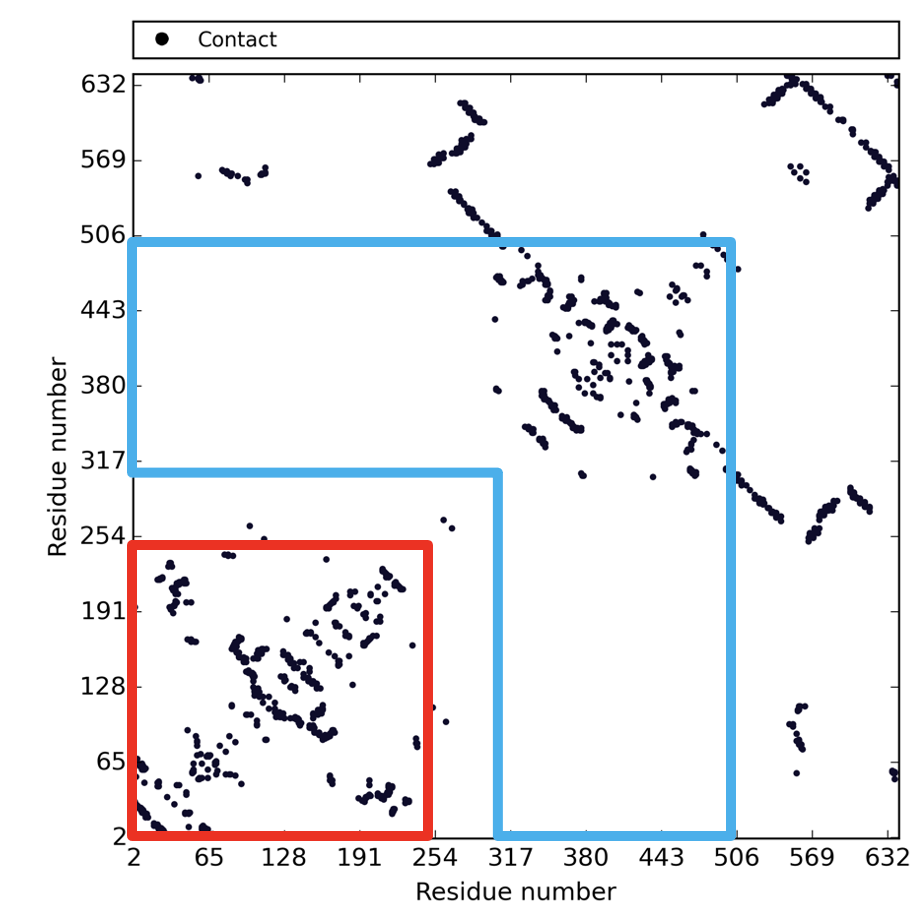
\includegraphics[width=\linewidth]{Results/5lil_1.png}
  \caption{5lilA contact map}
  \label{fig:0}
\end{subfigure}\hfil % <-- added
\begin{subfigure}{0.25\textwidth}
  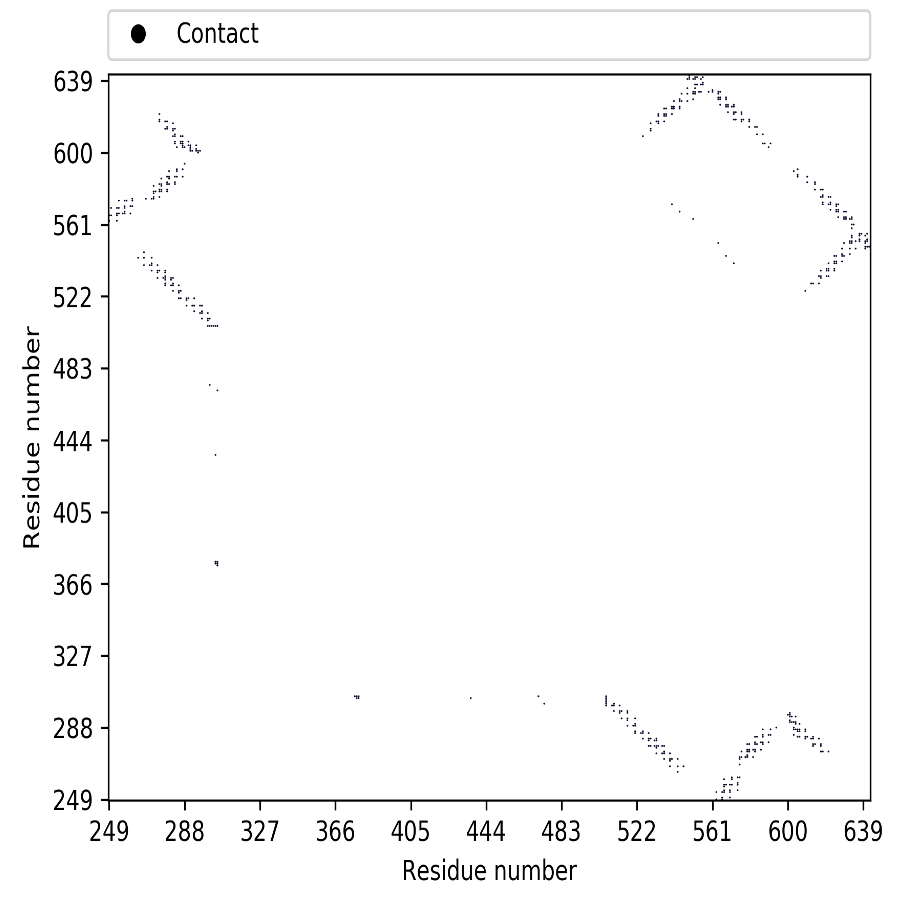
\includegraphics[width=\linewidth]{Results/5lil_2.png}
  \caption{Edited 5lil contact map}
  \label{fig:1}
\end{subfigure}\hfil % <-- added
\begin{subfigure}{0.25\textwidth}
  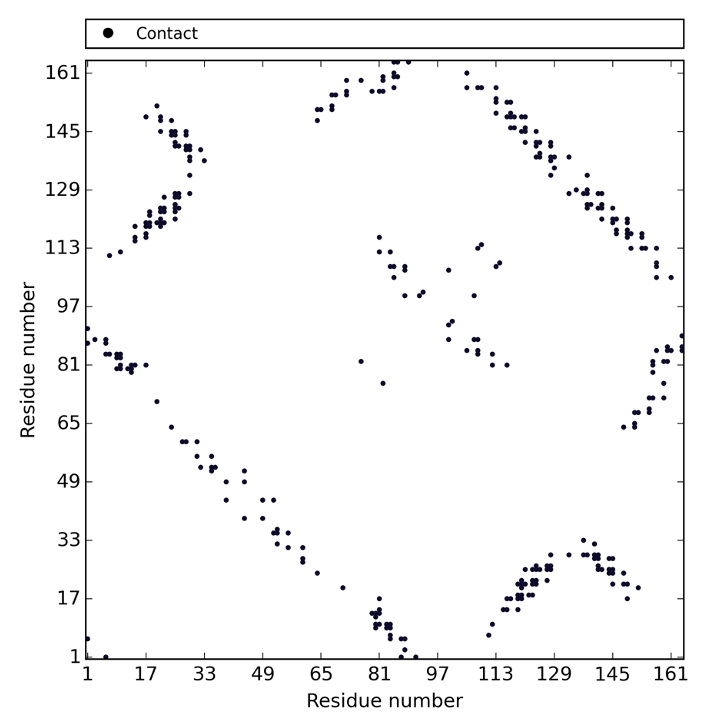
\includegraphics[width=\linewidth]{Results/5lil_topmodel.png}
  \caption{Top model contact map}
  \label{fig:2}
\end{subfigure}
\caption{5lil Contact map analysis}
\small
a) Blue box is periplasmic domain (residues 306-503) and red box is nucleotide binding domain (residues 1-240). b) 5lilA contact map with periplasmic and nucleotide biding domains removed. c) Rosetta membrane top model contact map.
\label{fig:5lil_cmaps}
\end{figure}

\begin{figure}[th!]
    \centering
    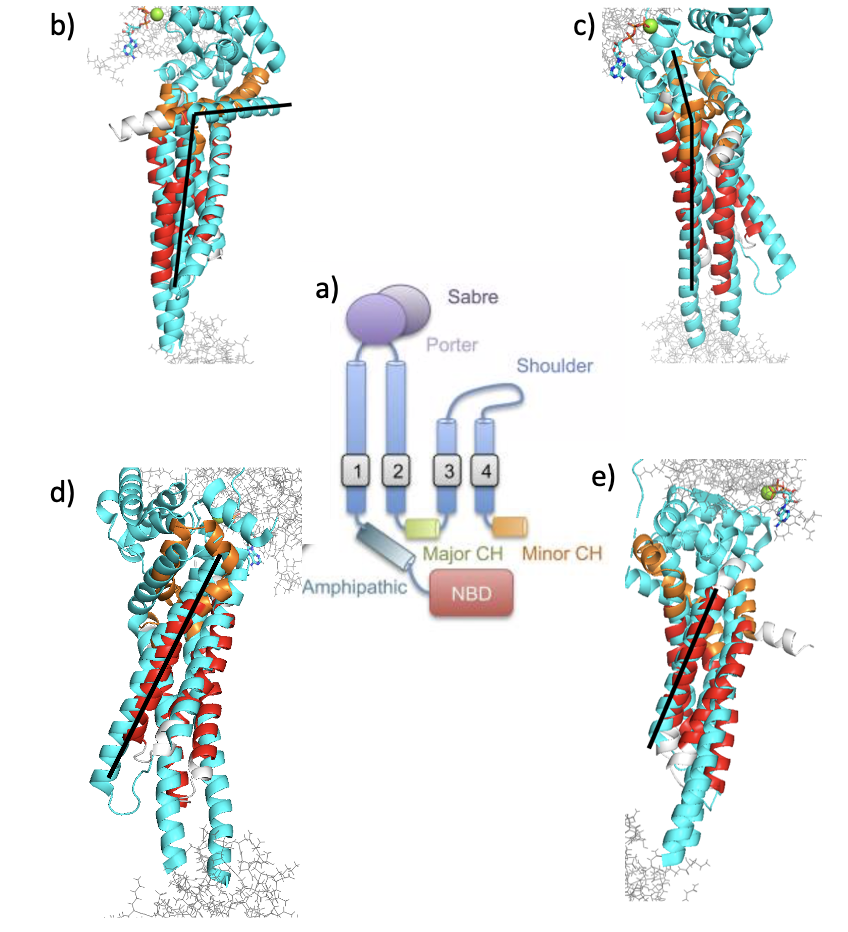
\includegraphics [width=100mm, scale =0.5]{Results/macb_fig.png}
    \caption{Structural alignment analysis of 5lilA and model.}
    \label{fig:5lil_schem}
    \small
    Cartoon: structurally aligned regions; Wire: non aligned regions. cyan: structural aligned region of 5lil; Red: regions of model that are predicted to be transmembrane helices by transmembrane topology prediction tools \ref{table:tm_pred}; Orange: regions of model where there is a lack on consensus between transmembrane topology prediction tools; White: Regions of model that are not predicted to to be transmembrane helices. 
    a)5lilA schmatic (adapted from \cite{pichoff2019roles}). b)Highlighted with a black stick is the alignment of model TM1 with TM1 of 5lilA (involved in dimer formation) along with the presence of the amphipathic helix. c) highlighted with a black stick is the alignment of model TM2 with TM2 of 5lilA (involved in dimer formation) Coupling helix 1 (CH1) (involved in NBD interaction). d)Highlighted with a black stick is the alignment of model TM3 with TM3 of 5lilA. e) Highlighted with a black stick is the alignment of model TM4 with TM4 of 5lilA and Coupling helix 1 (CH2) (involved in NBD interaction). 
\end{figure}

In spite of the fact that the resultant RosettaMembrane models appeared visually more promising; being more in line with transmembrane proteins and having good structural alignments with crystal structures of Type VI ABC transporters; once again when performing quantitative analysis of the ab initio models it resulted in poor precision scores (Figure \ref{fig:5lil_prec}). The unsuccessful modelling attempts lead to the detailed review of all sequence-based prediction data using custom visualisation plots.

\begin{figure}[th!]
    \centering
    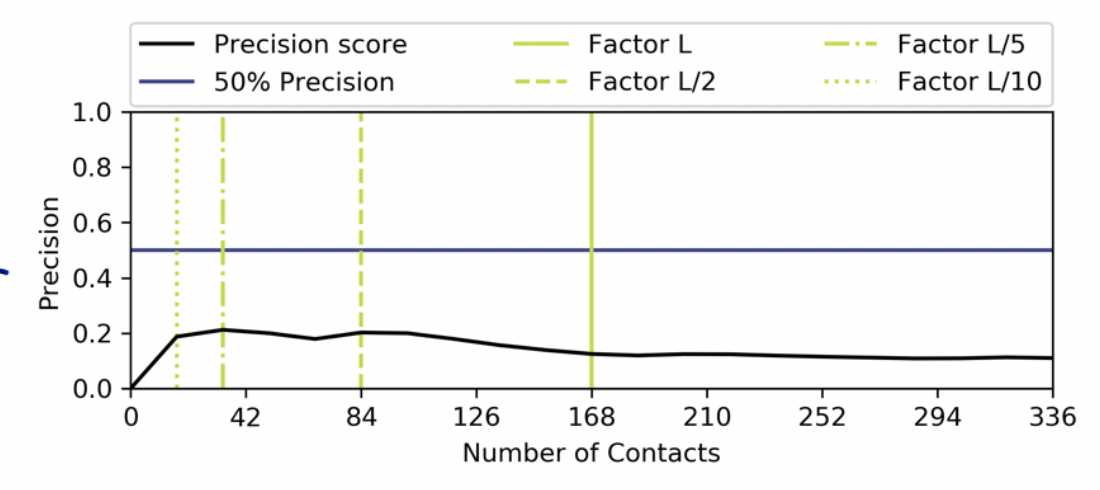
\includegraphics[width=100mm, scale =0.5]{Results/5lil_precision_fig.png}
    \caption{Precision profile for top RosettaMembrane model.}
    \label{fig:5lil_prec}
    \small
    Precision score evaluation of the RosettaMembrane model in relation to the predicted contacts at various contact cutoff values where L = sequence length (rounded down to the nearest whole number of contacts). The 50\% precision cut of is shown (blue line) as a visual marker. A minimum of 70\% contact satisfaction for the top L contacts would be suggestive of good quality models \cite{de2017comparing}.
\end{figure}

\newpage
\section{Development of ConPlot}
The poor precision scores of models built by Rosetta ab initio and RosettaMembrane, along with evidence that the transmembrane topology predictions may contain false positives (Table \ref{table:tm_pred}) led to the desire to visually cross-reference all available prediction data for both Mt2055 and Tmem41b. ConKit \cite{conkit2017}, a python interface to contact predictions, was chosen as a suitable platform to integrate various prediction data. ConKit was already able to output contact predictions in the form of a contact map where the contact predictions are visualised as a two-dimensional binary matrices \cite{godzik1993regularities}.  The contact maps traditionally have a blank space on and near the diagonal axis as they exclude contacts between sequential near neighbours. The ConKit software was adapted to parse other prediction data and output the data in a visual format with the contact map (figure \ref{fig:conplot}). The void in the diagonal of the contact map has been used previously to hold a visualisation of secondary structure information \cite{taylor2016algorithm}.  Various properties can be predicted by other sequence-based methods such as membrane and disorder predictions as well as residue conservation scores.  By integrating this multitude of data a more complete and integrated two-dimensional visual representation of the protein. \\

\begin{figure}[th!]
    \centering
    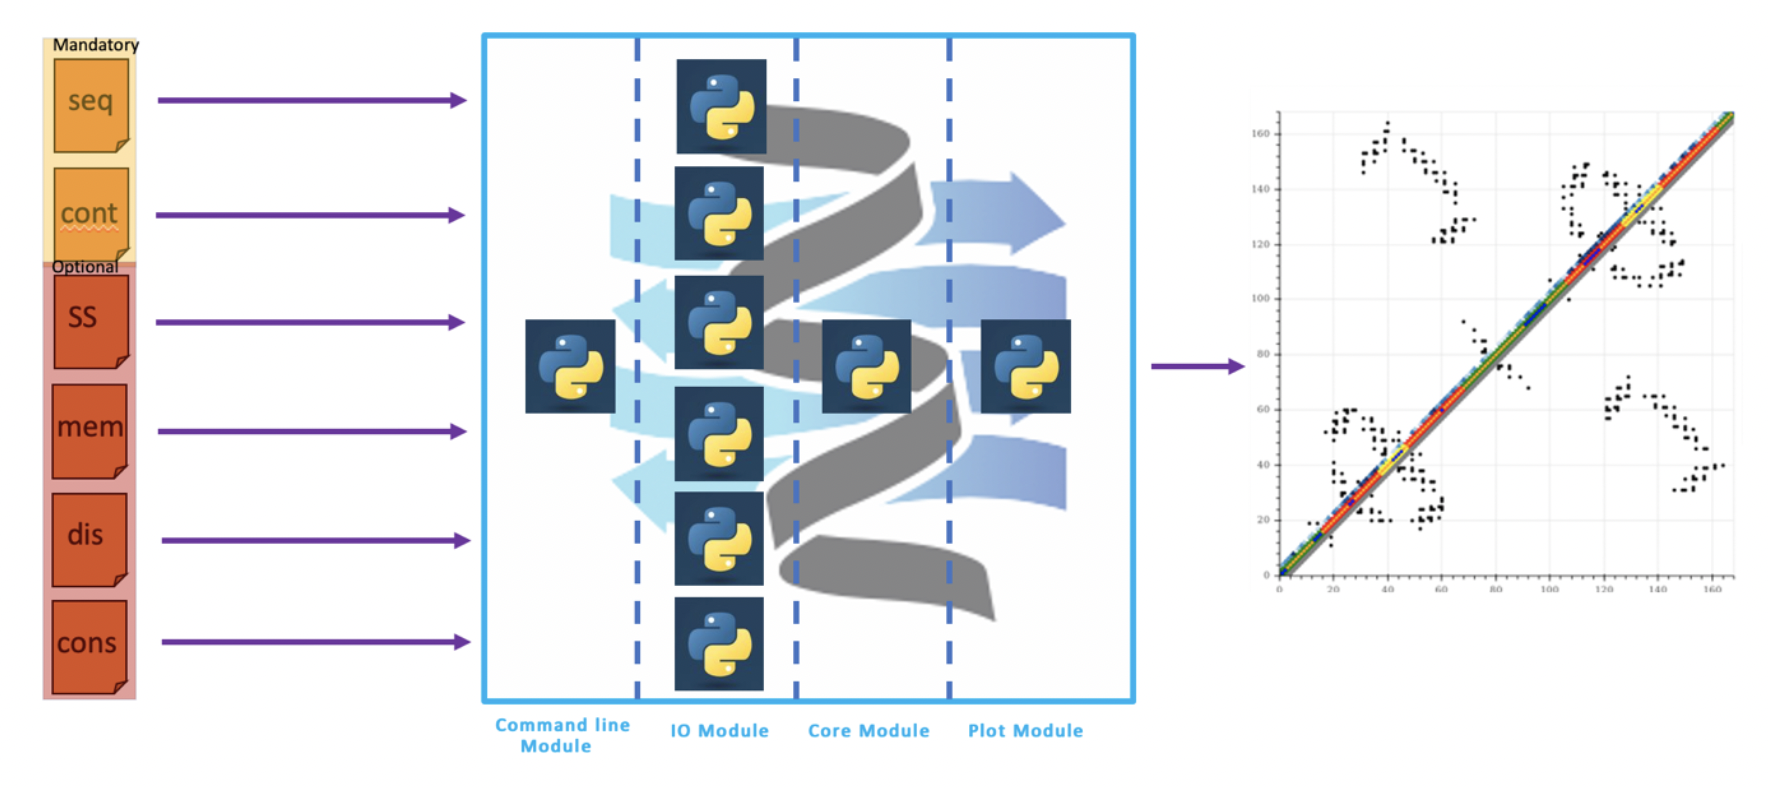
\includegraphics[width=\textwidth]{Results/conkit.png}
    \caption{Integration of new parsers into Conkit.}
    \label{fig:conplot}
    \small
    ConKit flow diagram showing prediction data types (left). Both the sequence data and contact information are mandatory sets of data required to build the data visualisation map; secondary structure (psipred format), membrane prediction (Topcons format), disorder prediction (Iupred2a format) and individual residue conservation scores (consurf format are optional data sets to be processed. New ConKit module scripts (middle) were constructed and integrated into the ConKit software. New output with prediction data visualised on diagonal (right) in the form of an interactive plot.
\end{figure}

New scripts were integrated into the command line, IO, core and plot modules of ConKit. The modifications to ConKit produced the desired output where all available prediction data for a given protein was displayed visually (figure \ref{fig:conplot}). (This visual cross referencing functionality was later developed into the web based application ConPlot \cite{sanchez2021conplot}).

With the visualisation of membrane predictions (TopCons) and secondary structure (PSIPRED) for Mt2055, inspection of the enhanced ConKit output revealed the possible presence of a re-entrant loop structure between residues 16–42 (Figure \ref{fig:w9_enhan_cmap}); a predicted transmembrane region (red) with a break in the centre that separates two distinct predicted helices (blue; from residues 16–25 and 28–42) in contact with each other). The predicted contact map also highlights a second re-entrant loop from residues 105–131, in accordance with the evidence that the protein family resulted from a tandem duplication. 

\begin{figure}[th!]
    \centering
    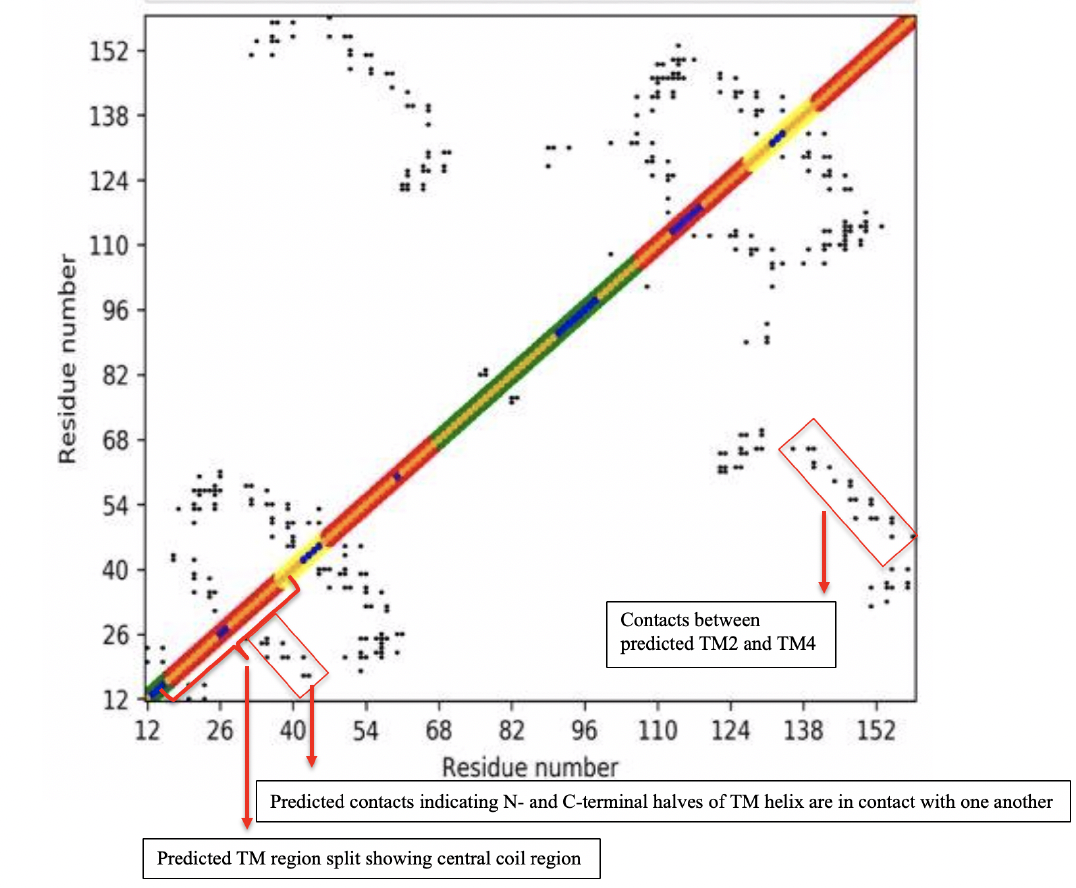
\includegraphics[width=\textwidth]{Results/enhanced_c_map_fig.png}
    \caption{Enhanced Mt2055contact map.}
    \label{fig:w9_enhan_cmap}
    \small
    Mt2055 Contact map constructed using DeepMetaPSICOV predictions with TOPCONS  membrane prediction & PSIPRED  secondary structure predictions overlaid. The outer diagonals show the TOPCONS membrane prediction (red regions being predicted TM helices, green; inside cell, yellow; outside). The thin central diagonal is the secondary structure prediction (orange, helix; blue, coil).
\end{figure}

Such a prediction would more obviously be treated as indicative of some kind of kink in the helix \cite{Law2016} but the explanation here is that these regions form re-entrant helices. A similar contact map feature can be easily generated from three transmembrane helices, however, this would result in a box feature of around 20x20 residues (and obviously reflected in the diagonal).  Since the re-entrant loop is making contact with itself this can only result in an approximately 10 residue antiparallel feature on the contact map.  Only approximately half of the transmembrane helix that is packed with the re-entrant helix will be making contact with the re-entrant loop, therefore, this would result in an additional 10 residue antiparallel feature in addition to a 10-residue parallel feature.  Together with the diagonal these will display an approximately 10x10 box feature (also reflected in the diagonal) on the contact map rather than the 20x20 box feature that three transmembrane helices (1 parallel pair and two anti-parallel ones) would produce (Figure \ref{fig:rent_cmap} ).  


\begin{figure}[th!]
    \centering
    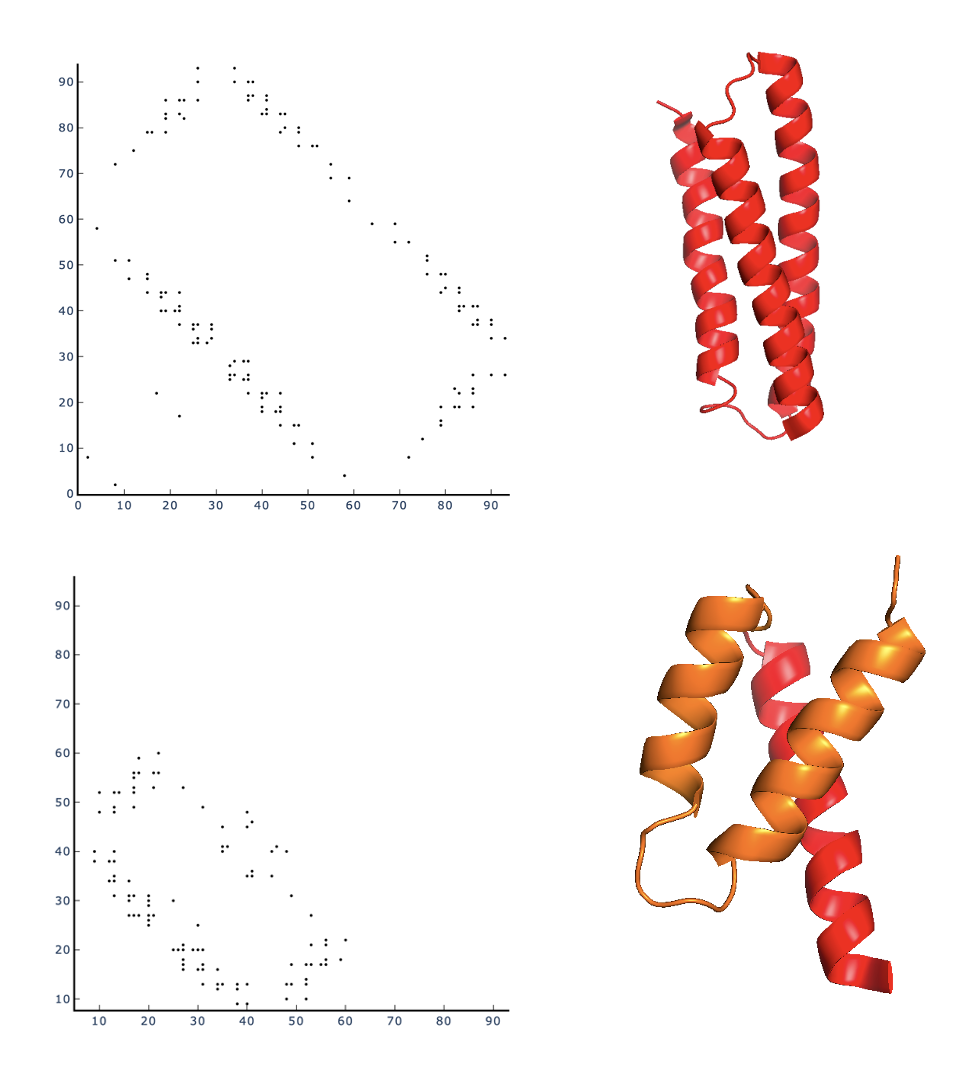
\includegraphics[width=\textwidth]{Results/rent_cmap.png}
    \caption{Re-entrant contact map.}
    \label{fig:rent_cmap}
    \small
    Top: Three transmembrane helix bundle (right) with its respective contact map (left); bottom: Re-entrant loop packed with a transmembrane helix (right) with its respective contact map (left).
\end{figure}

Similar contact map features, indicative of re-entrant loops packing against TM helices, can be seen clearly on the contact maps of other DedA proteins (data not shown). The MSA in Figure \ref{fig:msa} shows the relative positions of the re-entrant loops in their respective sequences.

Examination of the equivalent data for Tmem41b as well as the yeast homologue Tvp38 and two bacterial homologs YdjX and YdjZ revealed that all homologues contain a core consisting of an amphipathic helix, re-entrant loop and transmembrane helix in that order and inversely repeated (Figure \ref{fig:topology}). 

\begin{figure}[th!]
    \centering % <-- added
\begin{subfigure}{0.5\textwidth}
  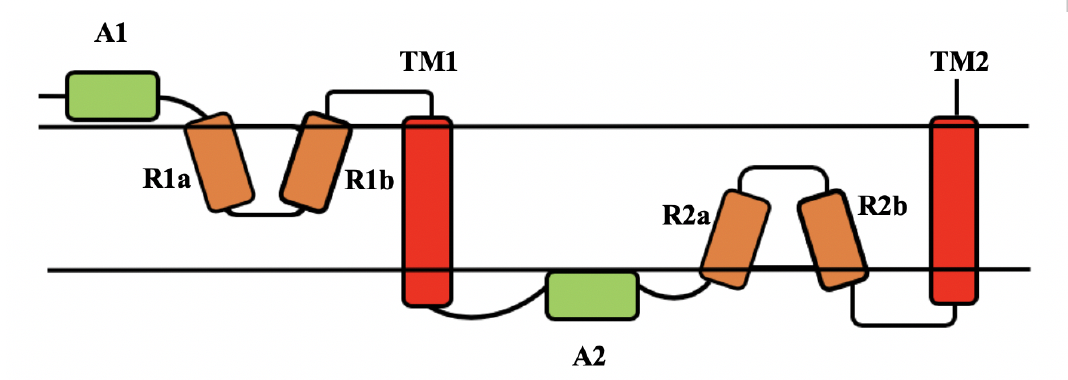
\includegraphics[width=\linewidth]{Results/w9_topology.png}
  \caption{Predicted topology for Mt2055}
  \label{fig:0}
\end{subfigure}\hfil % <-- added
\begin{subfigure}{0.5\textwidth}
  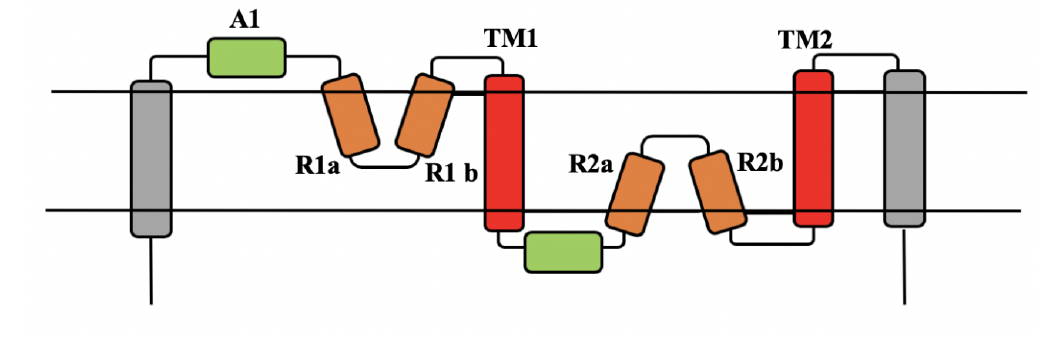
\includegraphics[width=\linewidth]{Results/tm_topology.png}
  \caption{Predicted topology for Tmem41b}
  \label{fig:1}
\end{subfigure}
\caption{DedA predicted topology}
\small
a) Predicted topology for Mt2055 based on contact, secondary structure, membrane & amphipathic predictions;
A1 – amphipathic helix 1; R1a (N-terminal half of re-entrant helix 1); R1a (C-terminal half of re-entrant helix 1; TM1- transmembrane helix 1; A2 – amphipathic helix 2; R1a (N-terminal half of re-entrant helix 2; R2a (Cterminal half of re-entrant helix 2; TM2- transmembrane helix 2.
b) Proposed topology for Tmem41b; A1 – amphipathic helix 1; R1a (N-terminal half of re-entrant helix 1; R1a (C-terminal half of re-entrant helix 1; TM1- transmembrane helix 1; A2 – amphipathic helix 2; R1a (N-terminal half of re-entrant helix 2; R2a (C-terminal half of re-entrant helix 2; TM2- transmembrane helix 2; with the presence of two-additional TM helices compared to Mt2055; Grey TM helices are additional helices to the core present in Tmem41b.
\label{fig:topology}
\end{figure}


\section{Advanced Modelling}
Alternative modelling software was identified that was not bound to membrane predictions and utilised a distance matrix approach rather than the use of the simpler quantal contact matrix restraints.  The modelling of Mt2055, Tmem41b and Yqja was executed using a locally installed version of trRosetta \cite{Yang2020} with default settings (figure  \ref{fig:trros_models}).

The Mt2055, Tmem41b and YqjA models had estimated TM scores of 0.633, 0.624 and 0.635 respectively, suggesting that they were likely to have captured the native fold of the family as a 0.5 cut off assumes generally the same fold \cite{zhang2005tm}. An all-against-all pairwise structural superposition of the models with DALI gave a mean Z-score of 11.9 confirming their strong similarity. The satisfaction of predicted contacts to validate the models (Figure \ref{fig:trros_models}) \cite{Simkovic2017} was also used to assess model quality. This showed that 80\% of the top L predicted contacts (where L is the length of the protein) were satisfied by the model contacts for both Mt2055 and YqjA and a value of 60\% was achieved for Tmem41b.  The high contact satsfaction scores are suggestive of good quality models \cite{DeOliveira2016}.  \\

Additionally, using ConPlot the superposition of the model contact map with the predicted contact map visually highlights the how close in alignment the two sets of contacts are (figure \ref{fig:w9_conplot}).\\

The models (Figure \ref{fig:trros_models}) confirmed the presence the predicted features: two inversely symmetrical repeated units each possessing a re-entrant loop (orange) packed with a TM helix (red).  In addition to this, the models also revealed that each repeating unit had a helix lying parallel to the membrane surface (green).\\

\begin{figure}[th!]
    \centering
    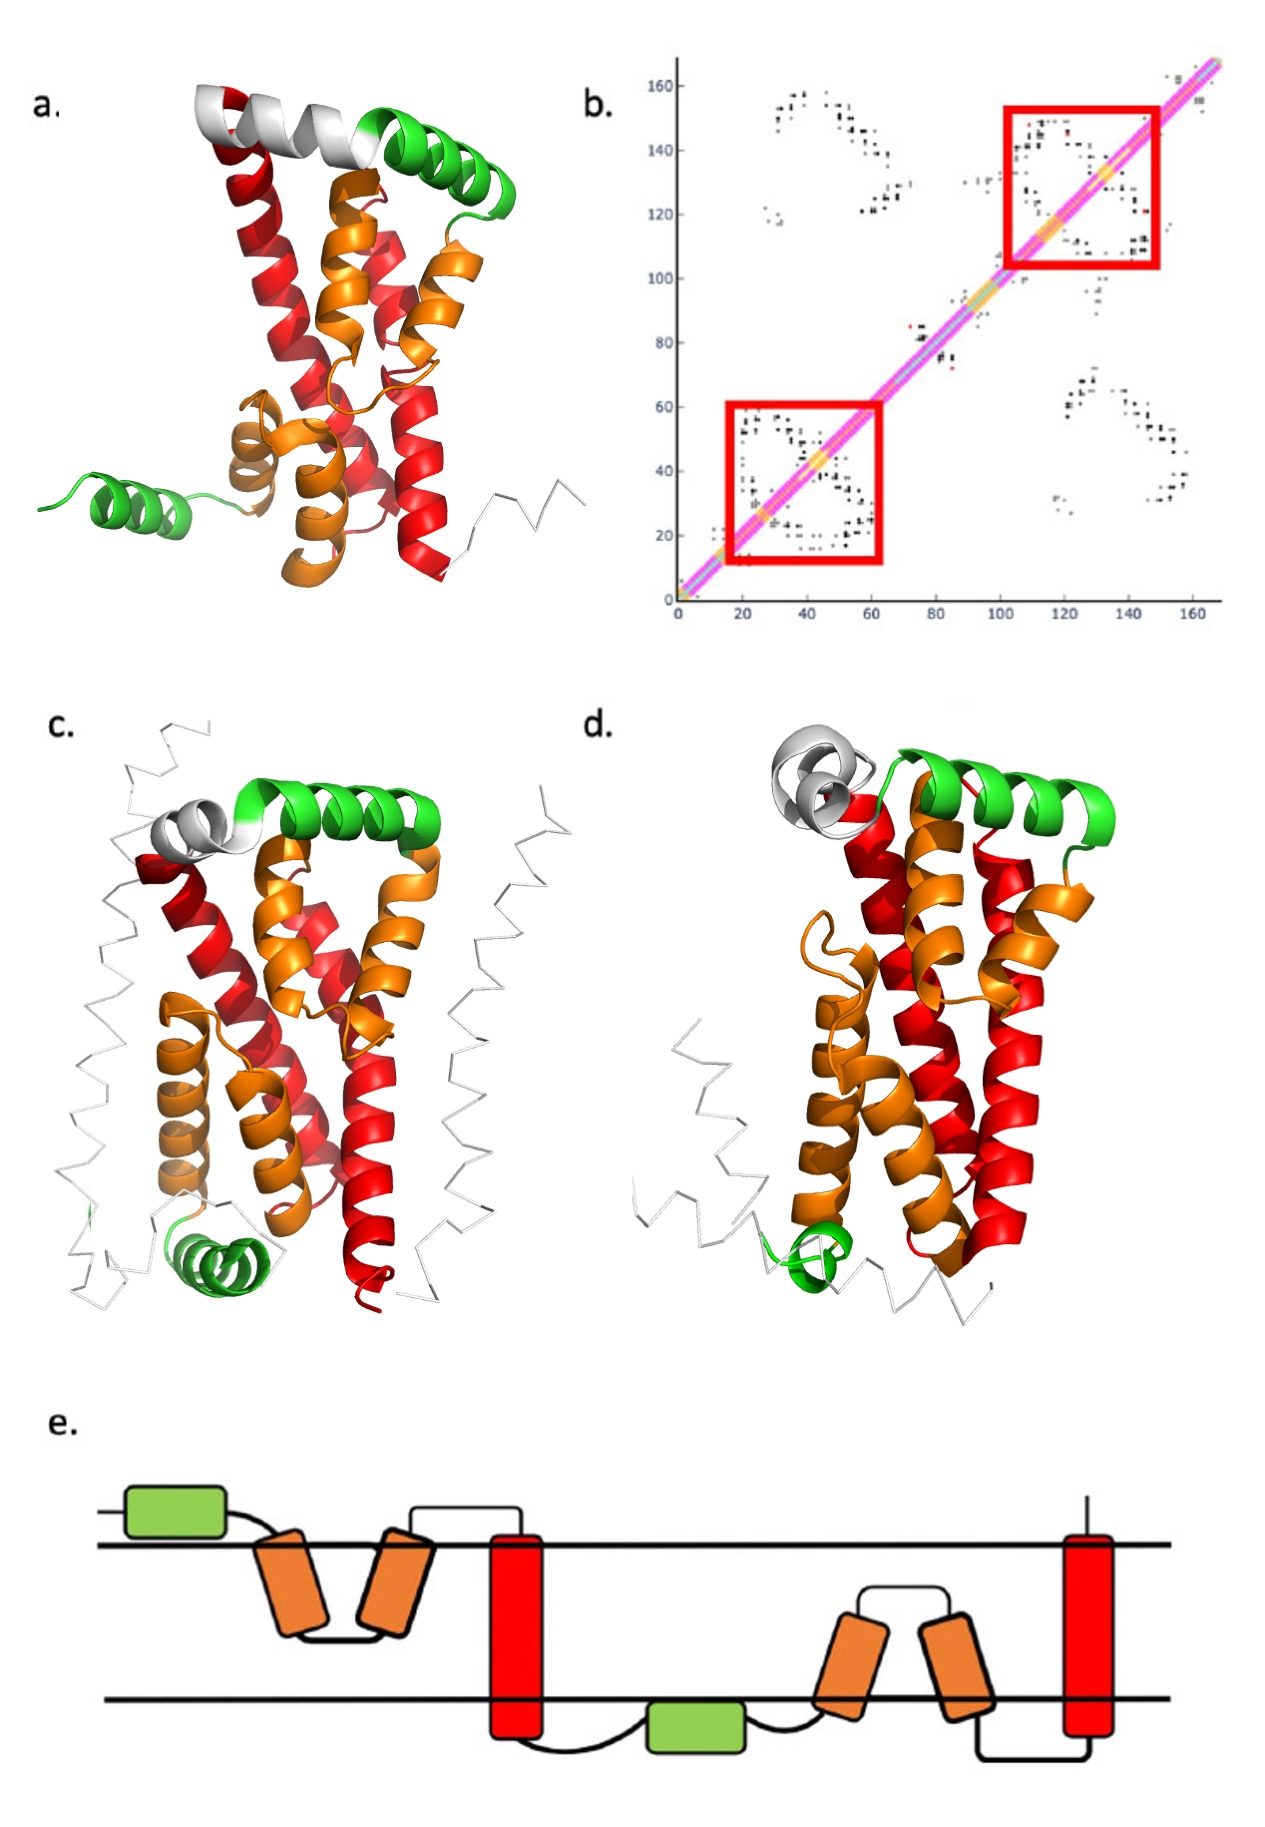
\includegraphics[width=100mm, scale =0.5]{Results/fig4.jpg}
    \caption{trRosetta Models}
    \label{fig:trros_models}
    \small
    (a) trRosetta model of MT2055 - amphipathic helix (green) and a re-entrant loop (orange) packed with a TM helix (red) (b) Superposition of DMP predicted contact map for Mt2055 and contacts from the Mt2055 model. Black points are matching contacts, red are mismatches and grey are contacts predicted but not present in the model. Diagonal is a visual representation of transmembrane helix and secondary structure prediction – central diagonal is the visualisation of the TopCons transmembrane prediction (orange being a TM helix) and the outer diagonals are the visual representation of the PSIPRED secondary structure prediction (pink – alpha helix and yellow – coil). Red boxes highlight the re-entrant loop and TM helix packing contact map signature. c) trRosetta model of Tmem41b only showing the conserved structural domain (residues 39-217) d) trRosetta model of YqjA only showing the conserved structural domain (residues 14-176). e) Proposed topology 
\end{figure}

\begin{figure}[th!]
    \centering
    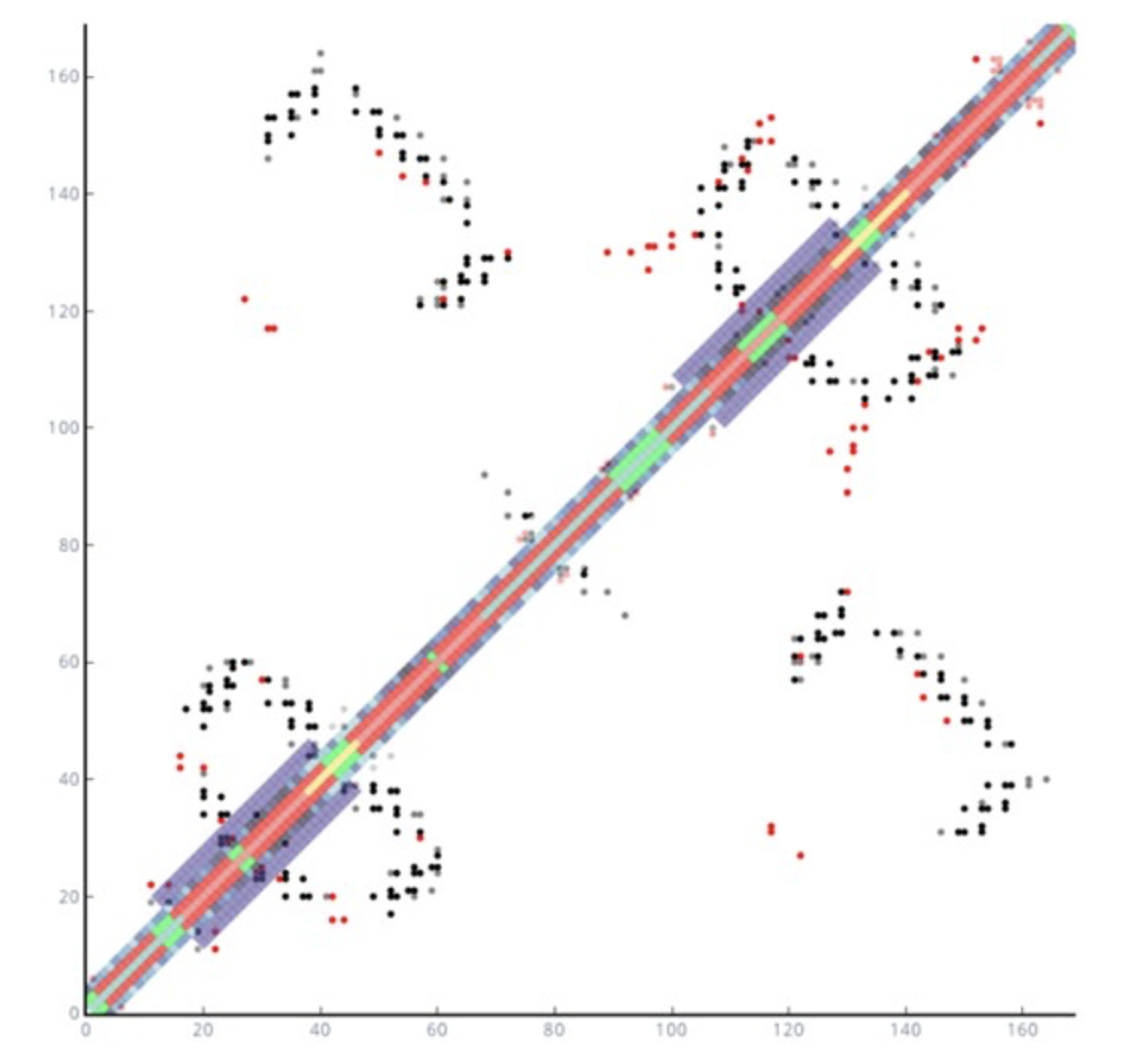
\includegraphics[width=100mm, scale =0.5]{Results/enhanced_c_map2.png}
    \caption{ConPlot Analysis}
    \label{fig:w9_conplot}
    \small
    Superposition of DeepMetaPSICOV predicted contact map with contacts present in the structure modelled with DMPfold. Black points indicate matches between the two maps, red points indicate contacts present in the model but not predicted and grey points are contacts predicted but not present in the model. Central track 0 in the diagonal is used for the TOPCONS transmembrane prediction (blue—outside cell, yellow—inside cell, light red—predicted transmembrane helix). PSIPRED secondary structure prediction is visualized by the tracks +1 and -1 adjacent to the centre of the diagonal (red—helix, green—coil). Tracks +2 and -2 represent CONSURF sequence conservation prediction (blue gradient, darker blue—more conserved, lighter blue—less conserved). Outermost tracks +3, -3, +4 and -4 were added using a custom file in which the location of the suspected re-entrant loops is highlighted in purple: between residues 16–42 and residues 105–131. 
\end{figure}


Further verification of local structures of the models was carried out. In order to test for whether the membrane-parallel helices (green in Figure \ref{fig:trros_models}) were amphipathic, an analysis of helical wheel diagrams for the fifteen residues preceding the putative re-entrant loops was performed with HELIQUEST \cite{Gautier2008}. The quantitative measures of the hydrophobic moment for the regions being analysed (Figure \ref{fig:heliquest}) support that they are indeed amphipathic helices. The hydrophobic moments ranged from 0.298 to 0.546 on a scale of 0-1.

\begin{figure}[th!]
    \centering
    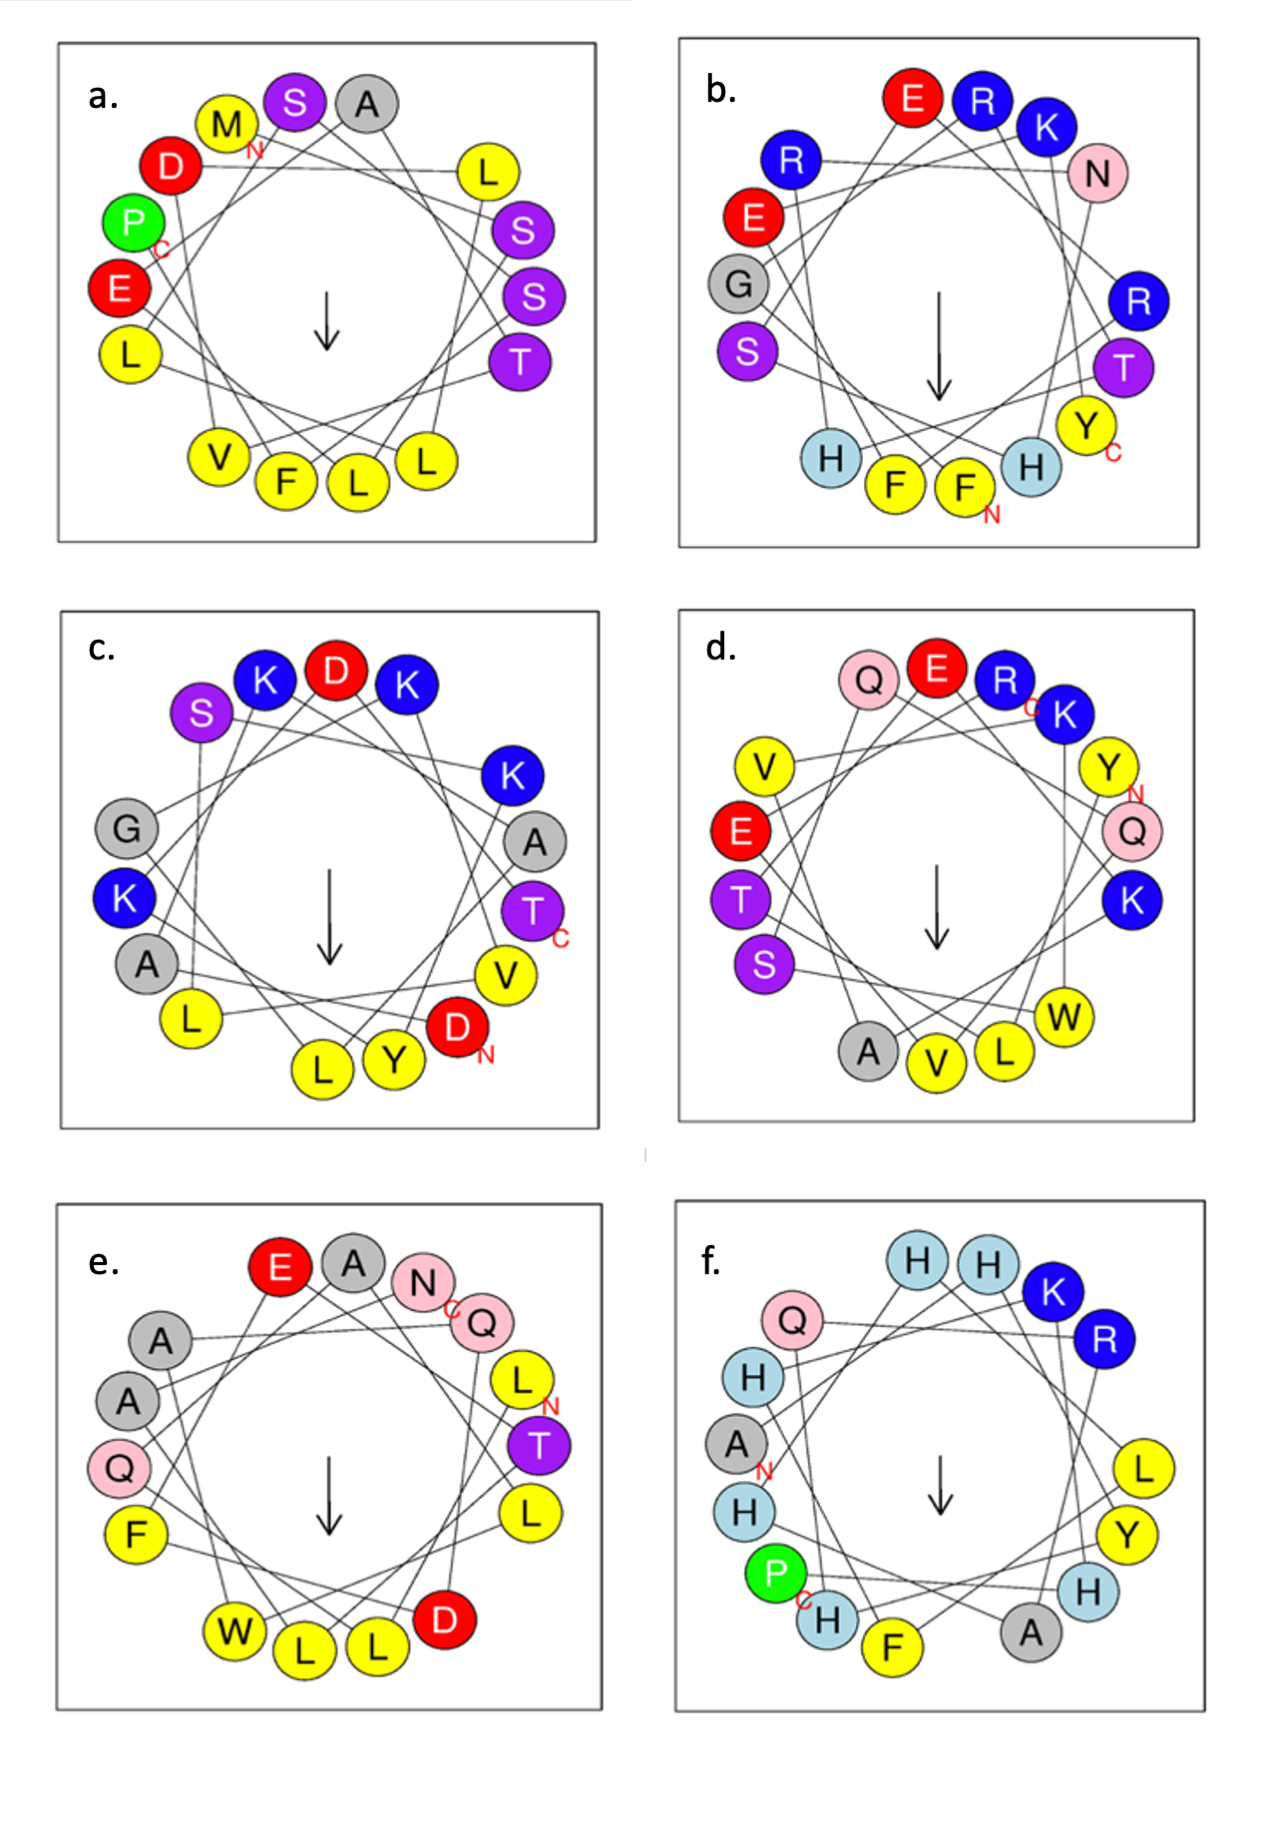
\includegraphics[width=125mm, scale =0.5]{Results/fig5.png}
    \caption{Helical wheel diagrams generated using the HELIQUEST server}
    \label{fig:heliquest}
    \small
    Hydrophobic residues are shown in yellow, serine and threonine in purple, basic residues in dark blue, acidic residues in red, asparagine and glutamine in pink, alanine and glycine in grey, histidine in light blue and proline in green circles. Arrows represent direction and magnitude of the hydrophobic moment and residue marked with ‘N’ is the N-terminal end of the putative amphipathic helix with the residue marked ‘C’ being the C-terminal end. (a) Mt2055 putative amphipathic helix 1 (hydrophobic moment of 0.298). (b) Mt2055 putative amphipathic helix 2 (hydrophobic moment of 0.546). (c) Tmem41b putative amphipathic helix 1 (hydrophobic moment of 0.471). (d) Tmem41b putative amphipathic helix 2 (hydrophobic moment of 0.420). (e). YqjA putative amphipathic helix 1 (hydrophobic moment of 0.295). (f) YqjA putative amphipathic helix 2 (hydrophobic moment of 0.396).
\end{figure}

The predicted presence of the amphipathic-re-entrant loop-TM helix features in DedA domain proteins prompted a desire to map sequence conservation on to the ab initio models. Using the CONSURF server to perform the mapping of sequence conservation onto the query models, it revealed that the re-entrant loop sequences are highly conserved. The high sequence conservation of re-entrant loops indicate that they are likely to be functionally and/or structurally important (Figure \ref{fig:consurf}).

\begin{figure}[th!]
    \centering
    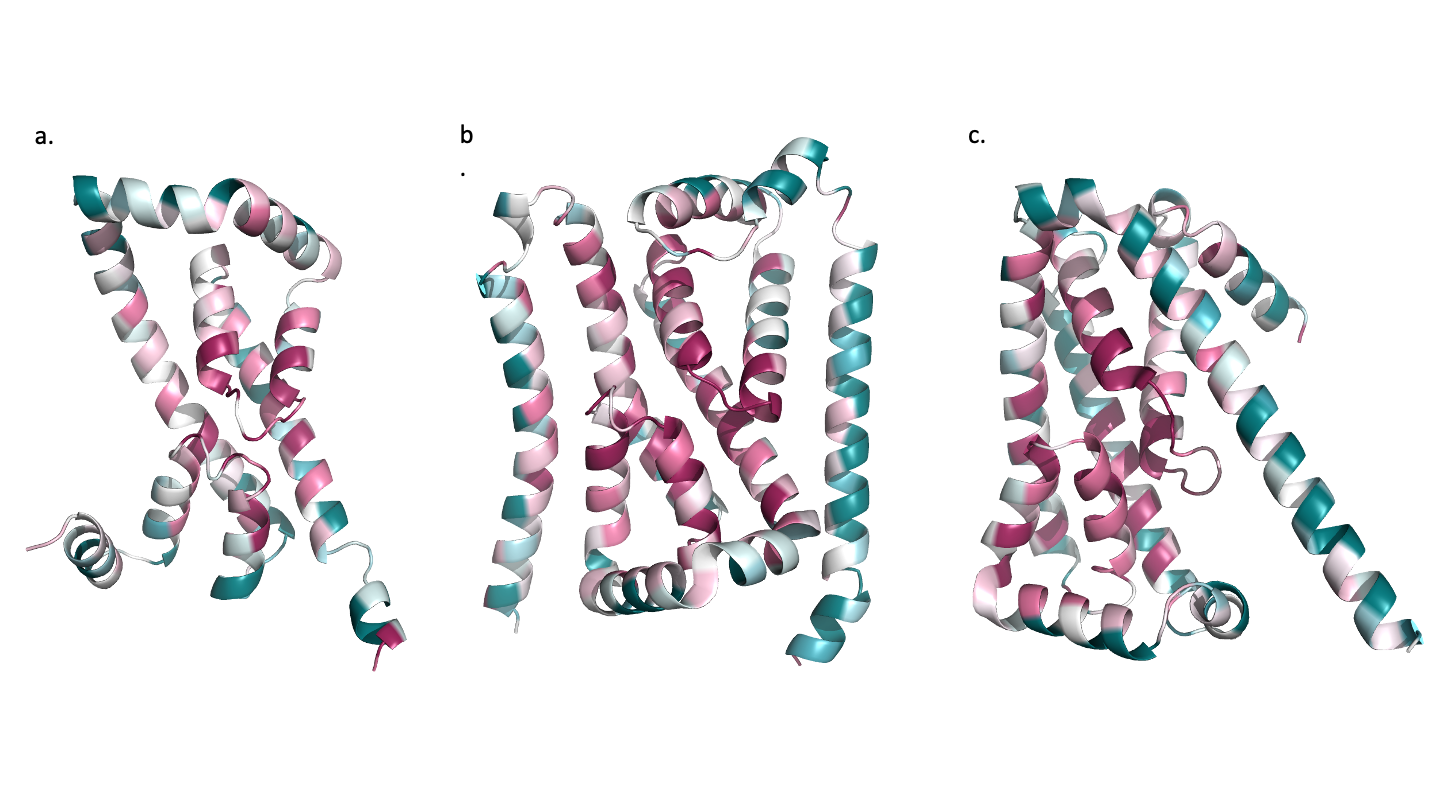
\includegraphics[width=\textwidth]{Results/fig6.png}
    \caption{CONSURF conservation mapping}
    \label{fig:consurf}
    \small
    trRosetta models with Consurf conservation mapping for (a) Mt2055 (b) Tmem41b (c) YqjA. Conservation is shown as a spectrum from purple (highly conserved) to blue (not conserved).
\end{figure}


Re-entrant loops were initially reported in the early 1990s in the cardiac Na\textsuperscript{+}/Ca\textsuperscript{2+} exchanger \cite{iwamoto1999unique}.
Since then re-rentrant loops have been detected in other membrane transporters and channels such as aquaporins \cite{de2001refined}, potassium channels \cite{zhou2001chemistry} and chloride channels \cite{dutzler2002x}.  The sequence-structure relationships of re-entrant loops have been studied before \cite{Yan2010} revealing that while TM helices have an even distribution of hydrophobic residues, re-entrant loops show an uneven distribution. Indeed, examination of the putative re-entrant loop sequences identified an inconsistent hydrophobicity distribution in both putative re-entrant loops of the homologues studied here (Figure \ref{fig:hydro_profiles}) with the C-terminal side being more hydrophilic. Interestingly it is the residues around the turning points of the re-entrant loops that more conserved (Figure \ref{fig:consurf}).  

\begin{figure}[th!]
    \centering
    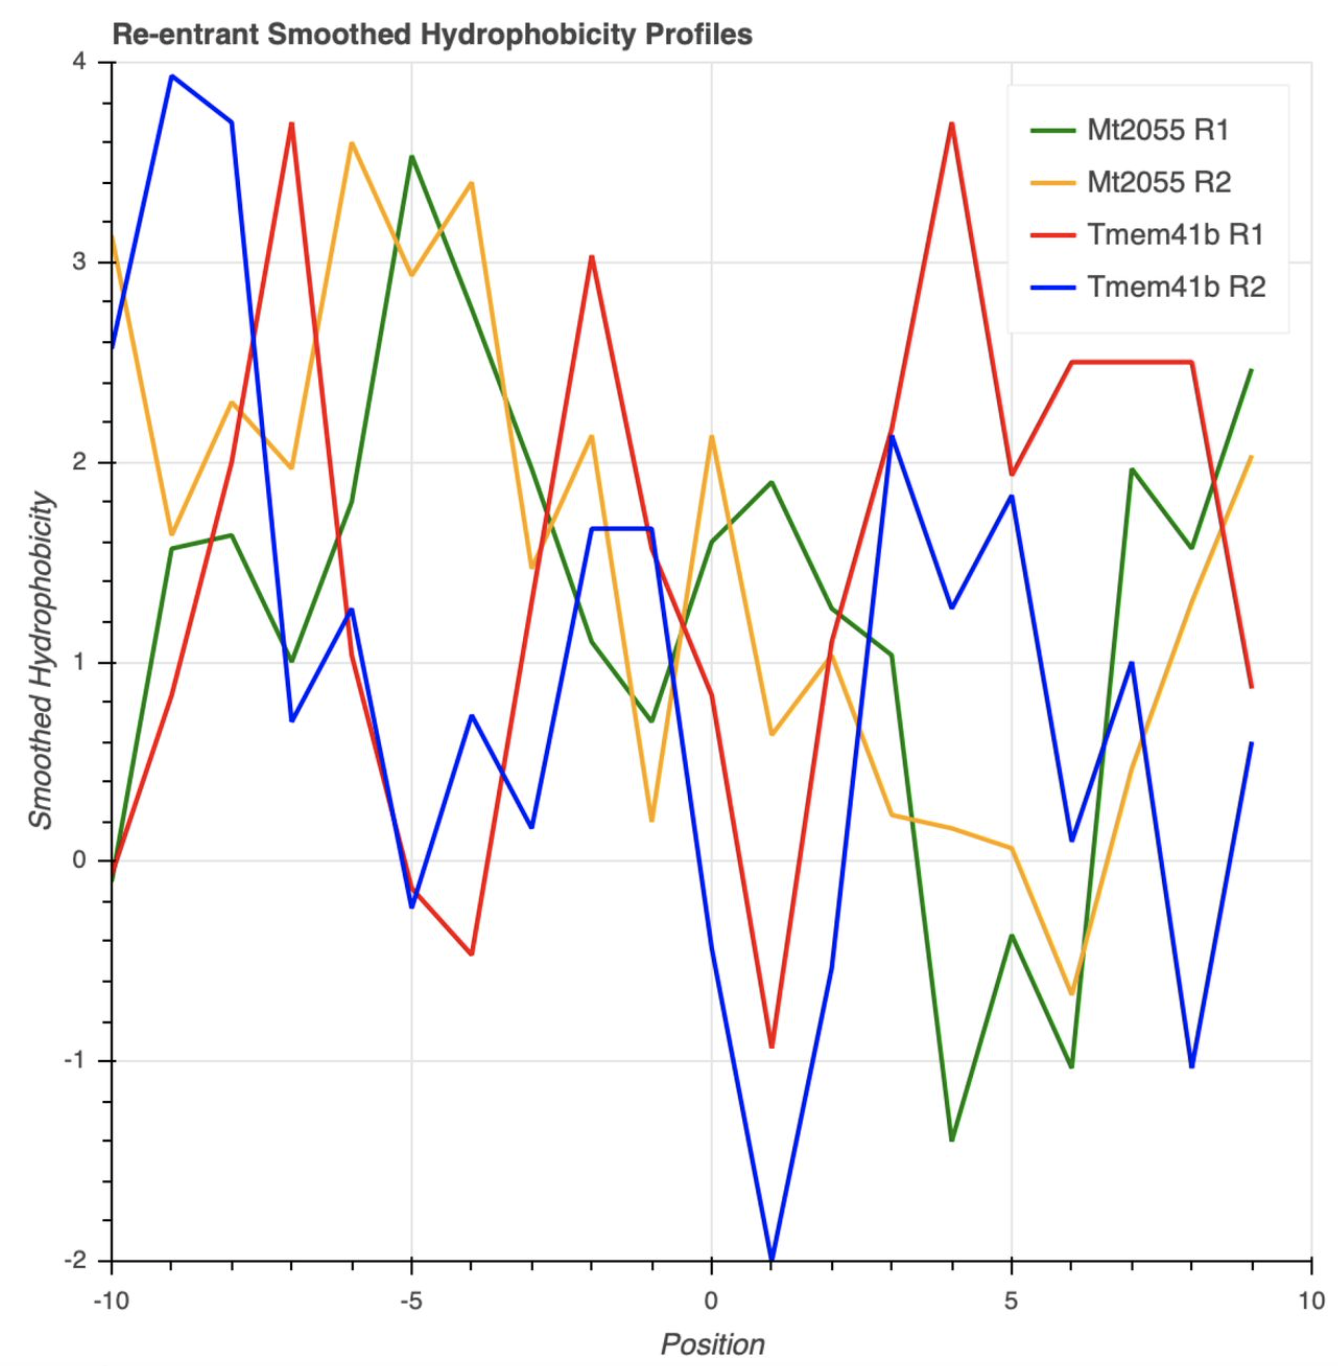
\includegraphics[width=125mm, scale =0.5]{Results/hydro_profiles.png}
    \caption{Re-entrant hydrophobic profiles}
    \label{fig:hydro_profiles}
    \small
    Smoothed hydrophobicity profiles for putative re-entrant loops of Mt2055 and Tmem41b. Smoothed the hydrophobicity distribution using a sliding window of three residues. For each position the mean hydrophobicity \cite{Kyte1982} of the three positions covered by the window is calculated and assigned to the position at the center of the window. Positions are numbered by assigning the central residue (proline; see later) as 0.
\end{figure}

Assessing the conservation across the sequence of PF09335/PF06695 homologues, ConSurf highlights regions of strong conservation. The strongly conserved regions are located in at the turning points of the re-entrant loops  and the mid-points of the tranmembrane helices that are packed against the re-entrant loops.  These regions come together in three-dimensional space. \\

In an effort to locate the presence of any functional residues the CONSURF data at the regions of highest conservation were examined. As expected from the sequence analysis, the conservation data identified the presence of proline residues at the ‘turning point’ of all putative re-entrant loops in the MSAs. Thus, the conserved proline identified above is suggested by the models to have a structural role providing the tight turn required for the approximate 20° (figure \ref{fig:angles}) angle making up the re-entrant loop.  


\begin{figure}[th!]
    \centering
    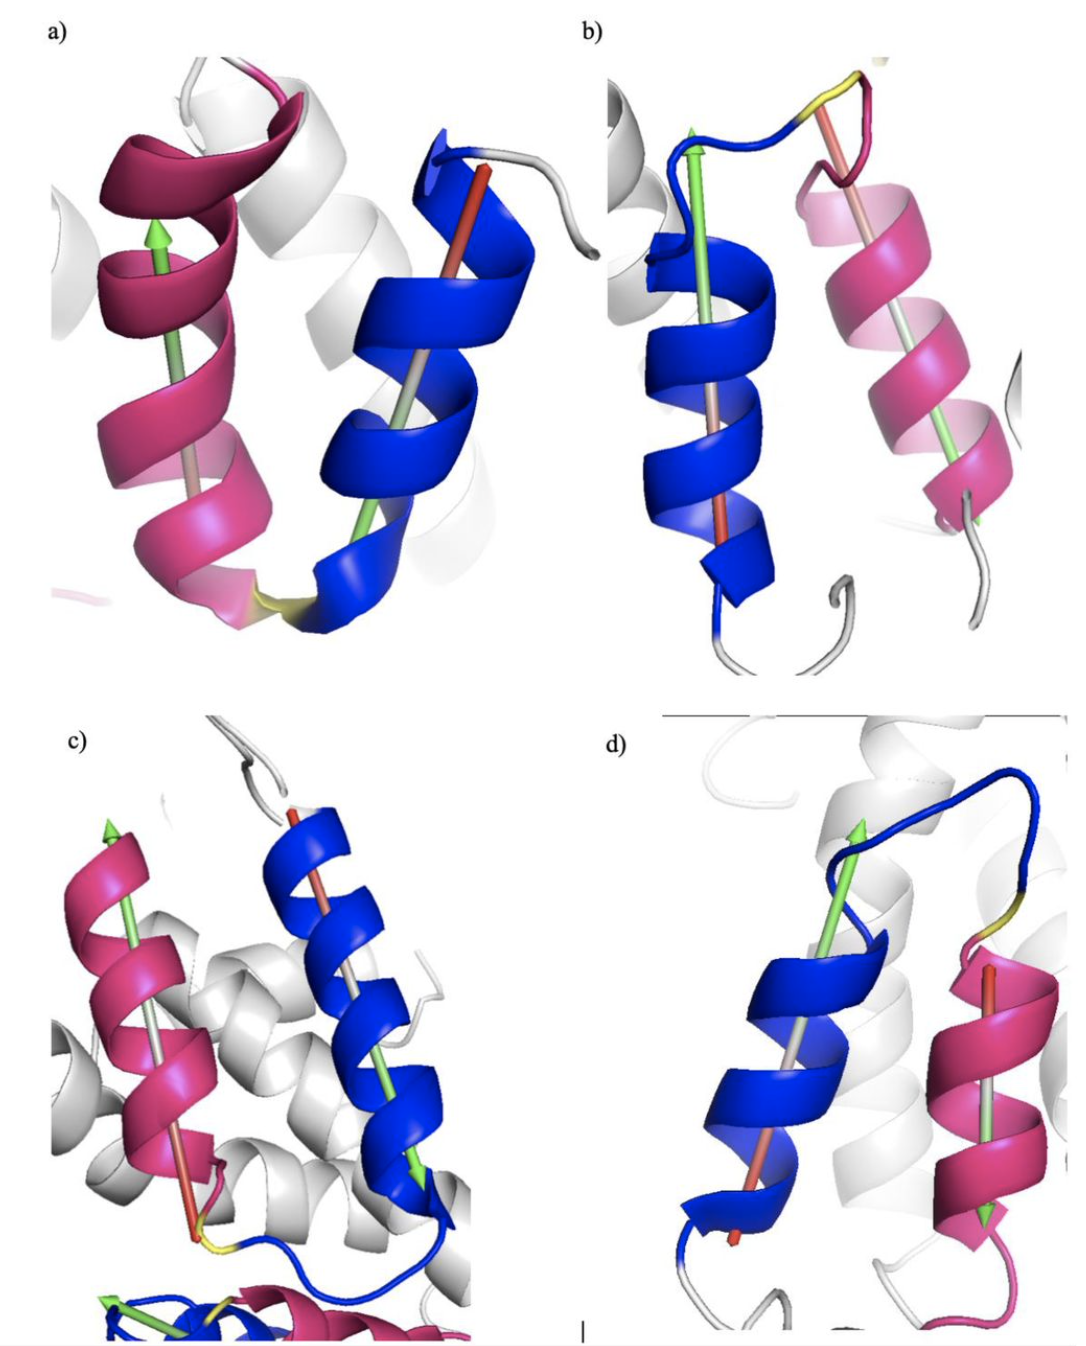
\includegraphics[width=125mm, scale =0.5]{Results/re_angles.png}
    \caption{Re-entrant angle measurements}
    \label{fig:angles}
    \small
    Tight re-entrant turn of around 160° a) Mt2055 R1 b) Mt2055 R2 c) Tmem41b R1 d) Tmem41b R2. Blue is C-terminal side of re-entrant loop, pink is N-terminal side of re-entrant loop, yellow is position of the proline. It can be seen that the proline residue is slightly off set from the turning point in some re-entrant loops possibly as a result of inaccuracy in the modelling.
\end{figure}

\section{Clustering of re-entrant loops}
The presence of re-entrant loops and the high density of conserved residues within them prompted an examination of experimentally characterised re-entrant loops in the PDBTM database. A total of 56 non-redundant re-entrant helices were identified (see Methods). All 56 were clustered with the putative re-entrant loops from Mt2055 and four PF09335 homologues (Tmem41b, Tvp38, YdjX and YdjZ) using relative E-values derived from an all-against-all BLAST run in CLANS \cite{Frickey2004} with a 0.1 p-value cut-off. The largest cluster contained 14 sequences, of which four were putative re-entrant sequences from the query proteins (Mt2055 C-terminal re-entrant, YdjX C-terminal re-entrant, Ydjz N-terminal re-entrant and YdjZ C-terminal re-entrant), seven (3org, 5tqq, 3nd0, 3det and 6coy) were re-entrant loop sequences from Cl\textsuperscript{-}/H\textsuperscript{+} antiporters, one was from a boron exchanger (5l25), one from an electron transporter (2n4x) [albeit classified as a member of the lysine exporter superfamily \cite{Saier2016}] and one from a mechanogated channel (5z10).\\

Analysis of the Cl\textsuperscript{-}/H\textsuperscript{+} antiporter structures show that they contain a similar inverted repeat as we infer for the DedA homologues, resulting in pseudo-2-fold axis of symmetry running along the membrane \cite{Duran2013}. Again similarly, the Cl\textsuperscript{-}/H\textsuperscript{+} antiporter 3orgA also contains the amphipathic helices on the N-terminal side of the re-entrant loops. The fact that the presence of the amphipathic helices is restricted only to 3orgA and not found in all homologues suggest that these features are not essential for function. A similar distribution of conservation is observed between the putative pore region of Tmem41b and the Cl\textsuperscript{-}/H\textsuperscript{+} antiporter 3orgA (Figure \ref{fig:3org}(d)). Analysing the sequence of all re-entrant loops of the top cluster (comprising members of the Tmem41b family and the transporters) revealed that they all contain a proline at the turning-point. \\

 
 
 A second clustering exercise was implemented where all re-entrant loops in addition to the proceeding 30 residues were extracted from a non-redundant re-entrant loop containing subset of the PDB. The resulting 193 library entries, supplemented with the re-entrant loop features from the ab initio models, underwent an all-against-all structural alignment utilising Dali. The Z-scores for these alignments were then used to cluster all the structures.  This screen resulted in the Mt2055, Tmem41b and YqjA re-entrant loop feature structures clustering with the re-entrant loop features of Cl\textsuperscript{-}/H\textsuperscript{+} antiporters; this was a similar result to the original sequence-based clustering; as expected all six re-entrant structures from the query models clustered together. The CLC transporter re-entrant structures of 3orgA (re-entrant 1 and re-entrant 2), 7bxu and 5tqq also clustered with the queries. Additionally, the re-entrant structure from an Undecaprenyl pyrophosphate phosphatase (UppP) (6cb2) also clustered with the queries. UppP is an integral membrane protein that recycles lipid and has structural similarities to CLC transporters \cite{Workman2018}. Contact maps derived from the pdb files of CLC and UppP structures show the contact map signature corresponding to the re-entrant/TM helix structural feature (data not shown). Interestingly, the UppP is more similar to the PF09335 family being only 271 residues in length and having only 6 TM helices with UppP being involved in phospholipid trafficking; a function possibly related to autophagosome construction which Tmem41b has been shown to be involved with. 
 \begin{figure}[th!]
    \centering
    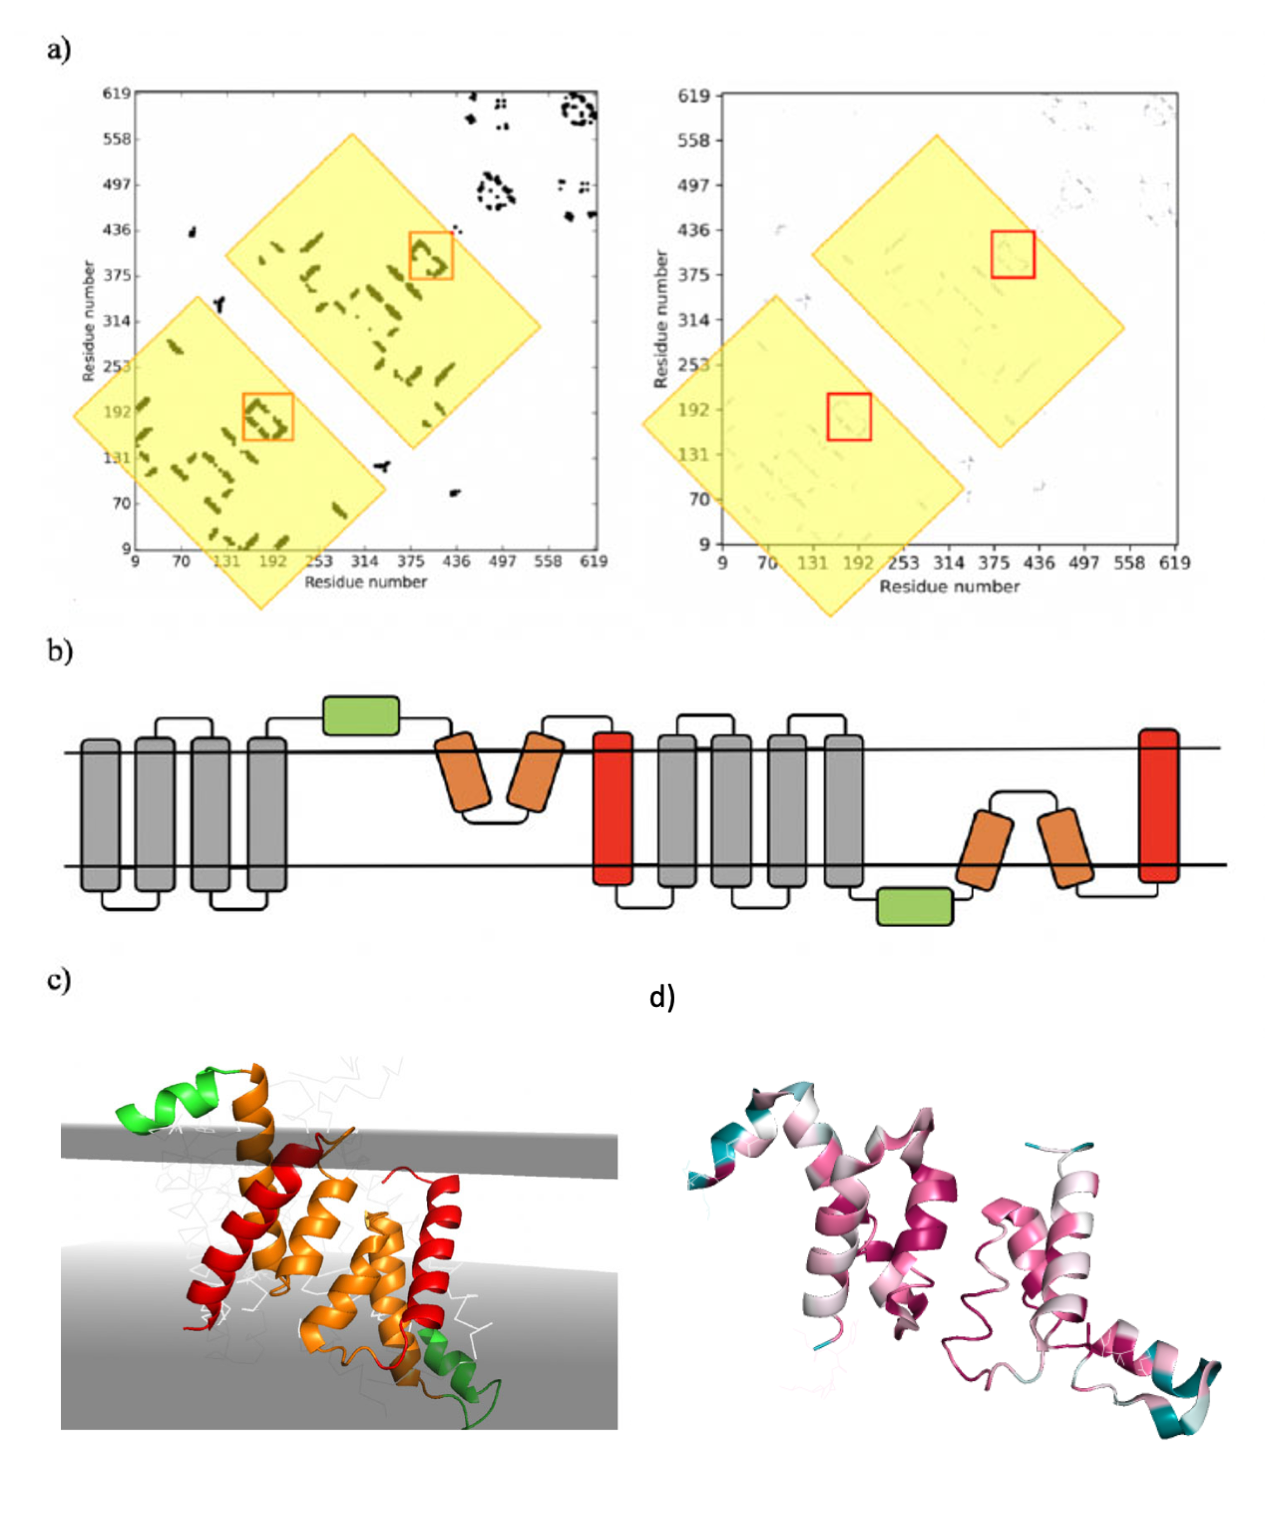
\includegraphics[width=150mm, scale =0.75]{Results/fig7.png}
    \caption{3orgA Analysis}
    \label{fig:3org}
    \small
    (a) Left - Predicted Contact map with repeating units highlighted in yellow boxes, contact map signature of re-entrant loop packed with TM helix in red boxes.; Right - The Experimental Contact map obtained from the PDB structure with repeating units highlighted in yellow boxes, contact map signature of re-entrant loop packed with TM helix in red boxes. (b) Actual 3orgA topology; grey: TM Helices that are additional to the core; red: TM helices contributing to the formation of the core; orange; re-entrant loops contributing to the formation of the core; green: amphipathic helices contributing to the formation of the core. (c) The 2-fold pseudo symmetry of the amphipathic/re-entrant loop/TM helix core inverted repeat structure of 3orgA with membrane positions shown as grey planes obtained from PDBTM.(d) Consurf conservation mapping on to the core inverted repeat structure of 3orgA.
\end{figure}

 In order to test whether 6cb2 predictions would generate the same contact map features as PF09335 and PF06695 homologues,  a TopCons \cite{Tsirigos2015} topology prediction was used to compare the predicted membrane topology of 6cb2 to its actual topology.  This exercise resulted in TopCons predicting false positive transmembrane helices at the positions of the re-entrant loops, as what was proposed for Tmem41b and homologues.  To investigate further, visual representations of the membrane topology from TopCons and the PSIPRED secondary structure prediction were plotted along the diagonal of the contact prediction for 6cb2 (Figure \ref{fig:6cb2_conplot}).  This clearly highlights that the N- and C- halves of the TopCons false positive predicted transmembrane helices in question were making contact with each other (by a length of around 10 residues).  Additionally, the secondary structure plot shows an interruption at the halfway point of the predicted transmembrane helices which would account for the abrupt change in direction of helix in the membrane.
 \begin{figure}[th!]
    \centering
    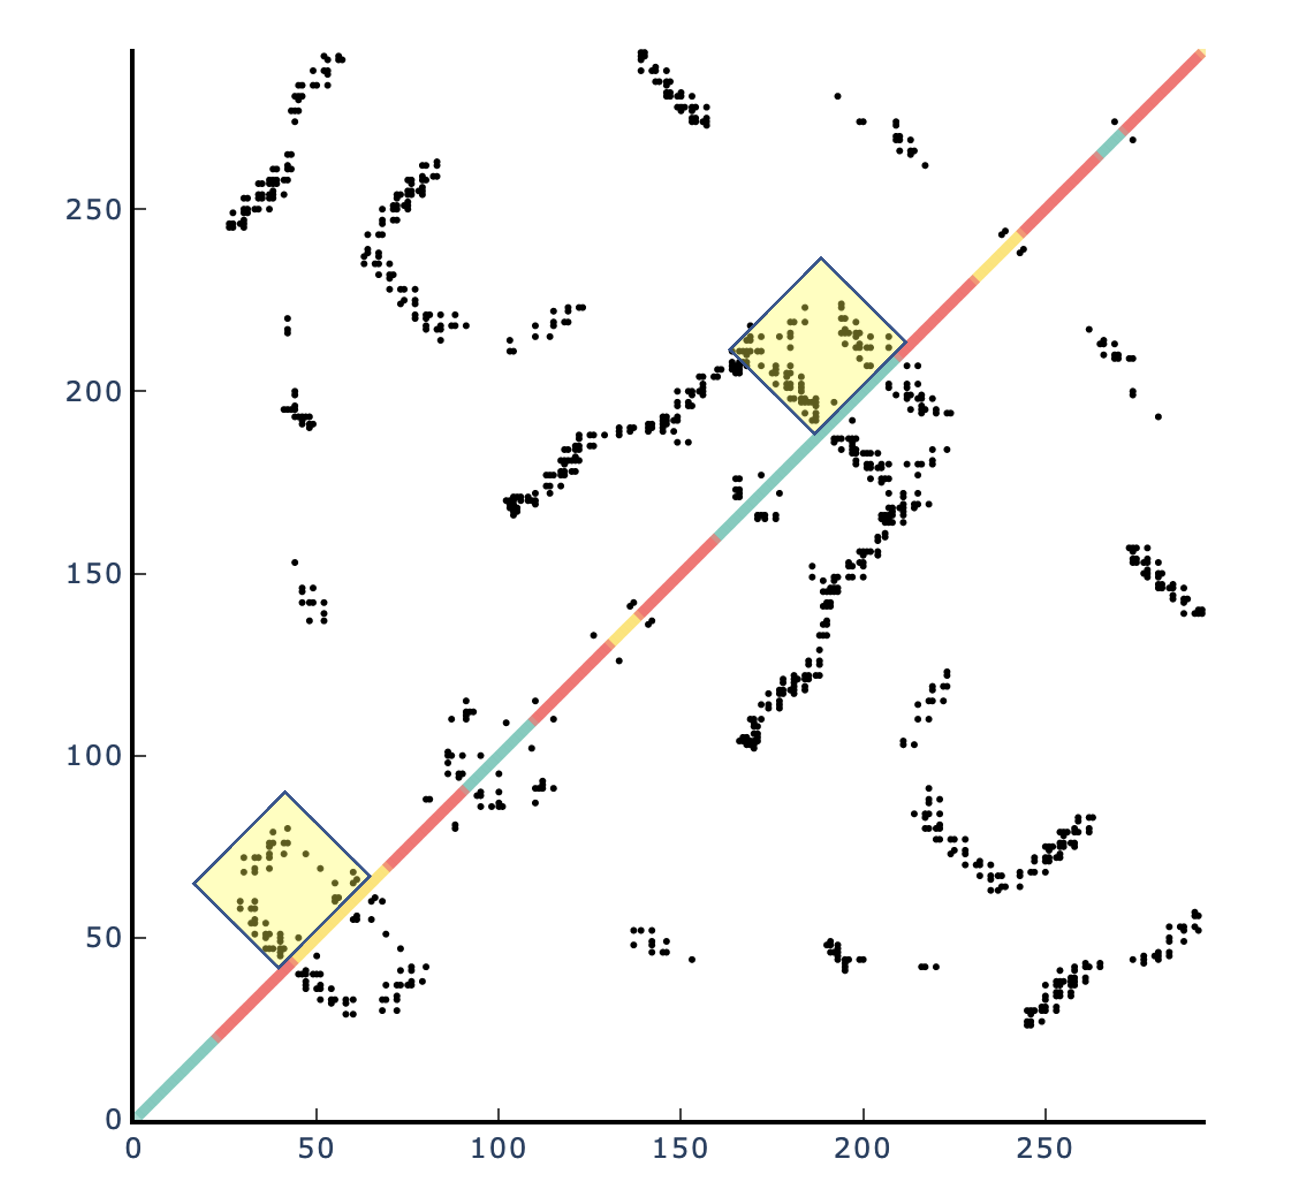
\includegraphics[width=\textwidth]{Results/6cb2_c_map.png}
    \caption{6cb2 Contact map}
    \label{fig:6cb2_conplot}
    \small
    Contacts for 6cb2 (black points) and a visual representation of the TopCons topology prediction (green -outside, red – TM helix, yellow-inside, yellow boxes are the re-entrant loop-TM-helix ‘signature’).  Cross-referencing the first re-entrant contact map  feature with the TopCons topology prediction it is clear that the TopCons topology must be wrong; the first TopCons predicted TM helix cannot be making contact with a region out-side of the membrane.  Indeed, examination of the crystal structure reveals that the contact feature highlighted does in fact result from a re-entrant loop packed with a TMhelix .
\end{figure}

A recent study has identified key residues (Figure \ref{fig:Yqja}) in the E. coli DedA protein YqjA that, when replaced in site directed mutagenesis experiments, resulted in properly folded (membrane localized) but non-functional proteins unable to complement alkaline pH sensitivity of E. coli YqjA mutant and antibiotic sensitivity of YqjA/YghB double mutant \cite{Panta2019}. Highlighting the essential residues (E39, D51, R130 and R136) on the YqjA model is striking as they come together in three-dimensional space with the N-terminal side of the first re-entrant possessing E39 and the C-terminal side possessing D51. R130 and R136 are similarly positioned on the second re-entrant loop (Figure \ref{fig:Yqja}). Re-entrant loops are known to form pores and here we have two proton-titratable residues (E39, D51) in close proximity to essential basic residues (R130 and R136) within a putative pore. This three-dimensional arrangement of key residues could serve a role in the coupling of the protonation status with the binding of a yet to be characterised substrate as is postulated for the multi-drug H\textsuperscript{+} antiporter MdfA \cite{Heng2015} where these same residues are located inside a central cavity.  

\begin{figure}[th!]
    \centering
    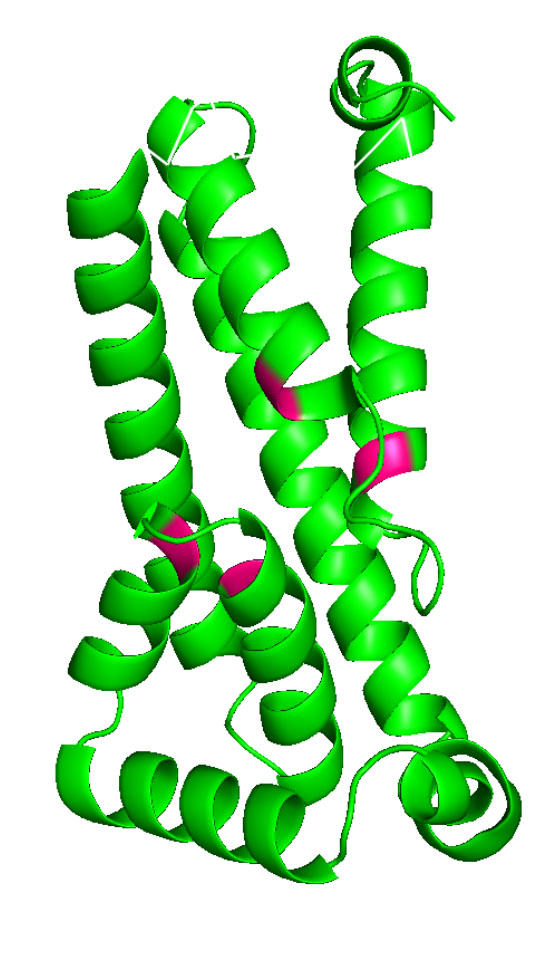
\includegraphics[width=50mm, scale =0.5]{Results/fig8.jpg}
    \caption{Annotated Yqja model}
    \label{fig:Yqja}
    \small
    Essential residues determined by SDM experiments highlighted in pink on a truncated YqjA model
\end{figure}

\section{Model Stability}
As it can be seen on Figure \ref{fig:3org}(c) that 3org contains additional helices that surround the interfacial helix - re-entrant loop - transmembrane motif. Indeed 3org forms a dimer, where the dimer interfaces are formed by the re-entrant loops and the additional transmembrane helices that surround this core. This arrangement ensure the lipid embedded structure is energetically stable \cite{Feng2010}. In the proposed model for the PF09335 and PF06695 homologues, the re-entrant loops are not wrapped by other helices thus lipids may interact them; this could be energetically unfavorable.  However, the shielding of the re-entrant loops produced by this wrapping could be achieved in Tmem41b and other family members by a similar dimerization as seen in 3org. Indeed, homodimers and higher oligomers have been detected experimentally in \emph{E. coli} YqjA \cite{Keller2015, scarsbrook2021topological}. Furthermore, submission of all three of the final models to the DeepHomo server \cite{yan2021accurate} reveals the clustering of moderately strong contact predictions (with a reliability > 0.5) that are not satisfied by the 3D monomeric structure and hence are consistent with homomeric intermolecular interactions being conserved across the family (figure \ref{fig:deephomo}). 

\begin{figure}[htb]
    \centering % <-- added
\begin{subfigure}{0.5\textwidth}
  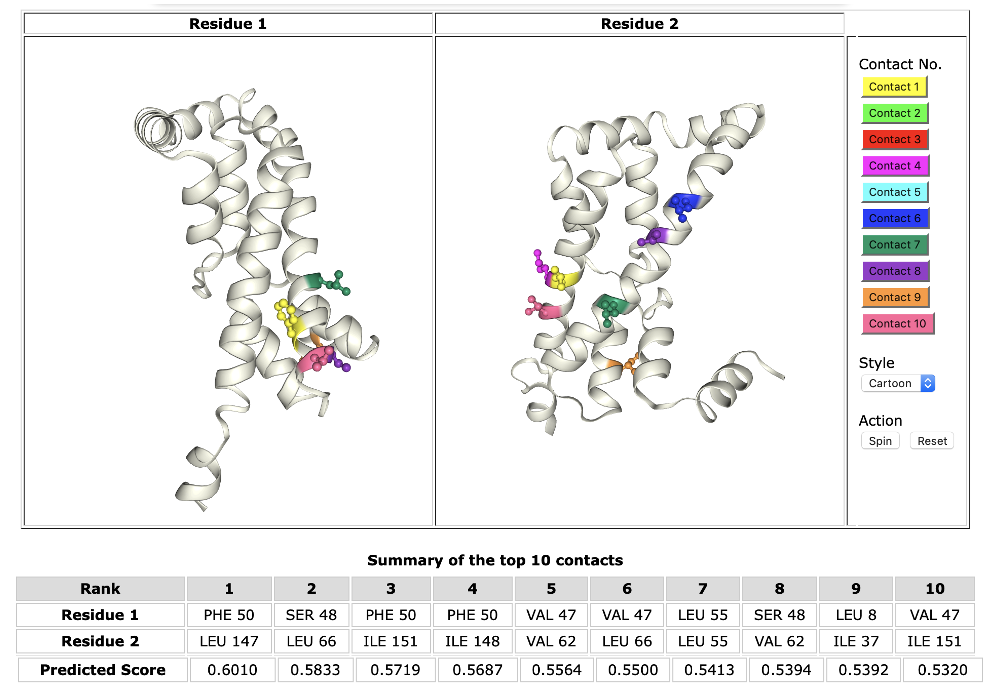
\includegraphics[width=\linewidth]{Results/w9_deep_homo.png}
  \caption{DeepHomo results for Mt2055}
  \label{fig:0}
\end{subfigure}\hfil % <-- added
\begin{subfigure}{0.5\textwidth}
  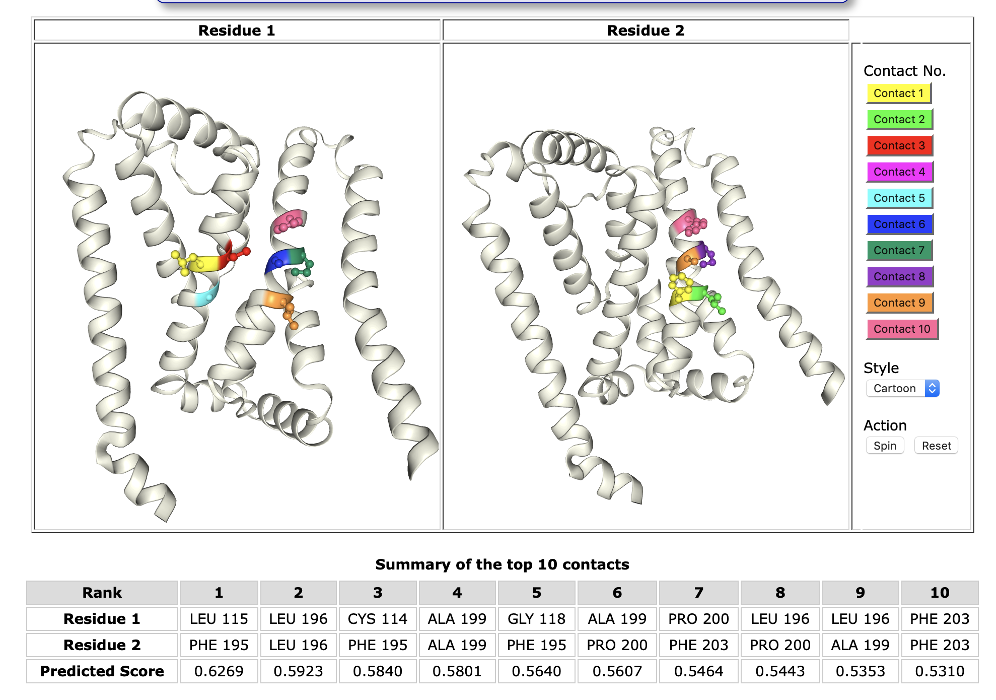
\includegraphics[width=\linewidth]{Results/tm_deephomo.png}
  \caption{DeepHomo results for Tmem41b}
  \label{fig:1}
\end{subfigure}
\caption{DeepHomo Results}
\small
The figure depicts two identical monomers displayed side-by-side, highlighting two corresponding residues involved in a contact. Summary of rankings and residue pairs for the top 10 contacts are displayed. The predicted scores range from 0.0 to 1.0, where higher scores indicate a higher likelihood of contact between the residue pairs.
\label{fig:deephomo}
\end{figure}

\section{AlphaFold2 Modelling}
The recent release of AlphaFold2 (AF2) \cite{Jumper2021} provided another opportunity to model Tmem41b and related proteins.  AF2 constructed models that support the trRosetta monomer predictions (Figure \ref{fig:w9_af}); aligning each of the trRossetta models for Mt2055, Tmem41b and YqjA with their respective AF2 counterparts yielded Z-scores of 18.4, 21 and 19.4 respectively.  Figure \ref{fig:af2_modelling} provides a visual insight of how the DedA domain modeling evolved during the period of this PhD; displaying the output models from the three incarnations of Rosetta to an AF2 model. 

Attempts to model homodimers of Mt2055 utilising the multimer mode of AF2 proved unsuccessful; chains of the output models did not come together to form an interface.  


\begin{figure}[htb]
    \centering % <-- added
\begin{subfigure}{0.25\textwidth}
  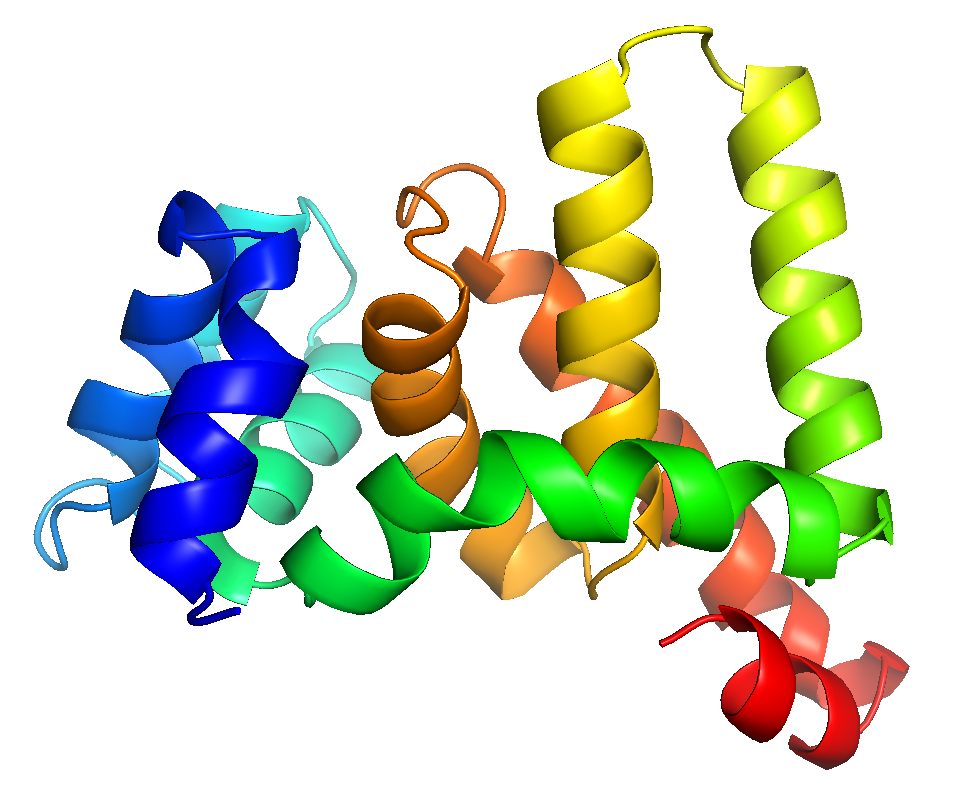
\includegraphics[width=\linewidth]{Results/w9_ros.png}
  \caption{Rosetta ab initio Mt2055 model}
  \label{fig:w9_ros}
\end{subfigure}\hfil % <-- added
\begin{subfigure}{0.25\textwidth}
  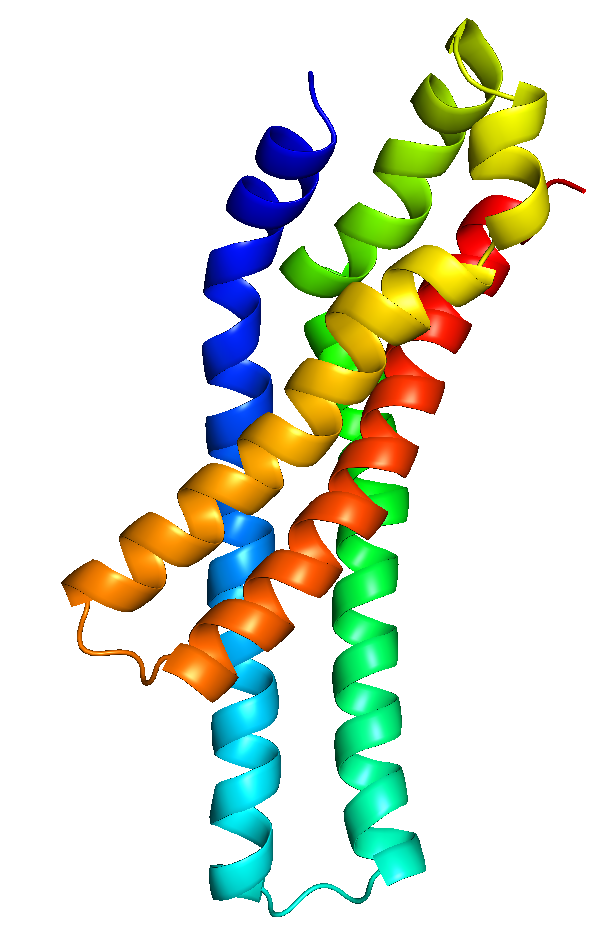
\includegraphics[width=\linewidth]{Results/w9_rosM.png}
  \caption{RosettaMembrane Mt2055 model}
  \label{fig:w9_rosM}
\end{subfigure}
\begin{subfigure}{0.25\textwidth}
  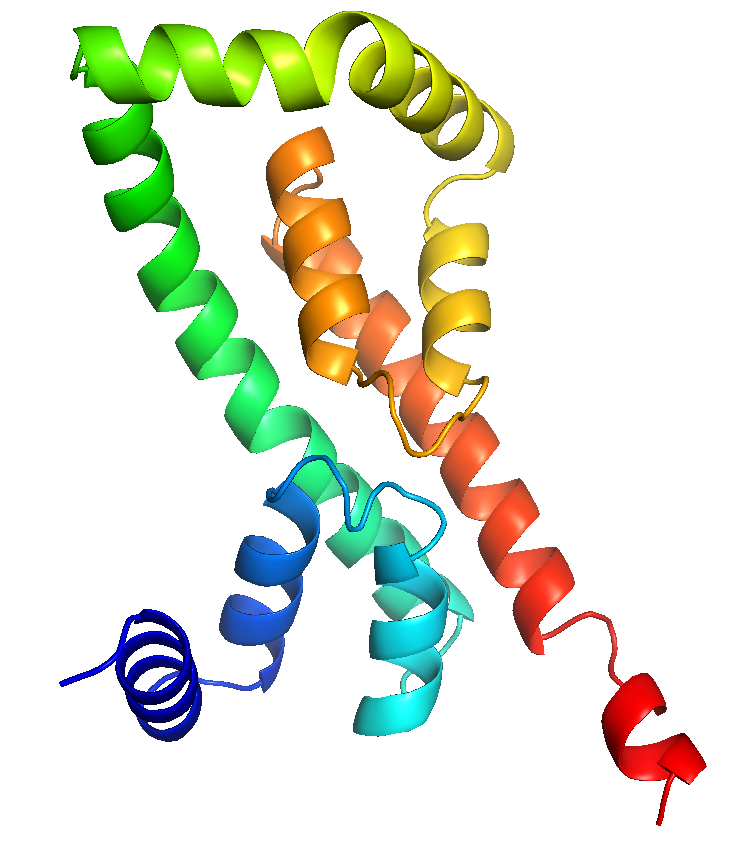
\includegraphics[width=\linewidth]{Results/w9_tr.png}
  \caption{trRosetta Mt2055 model}
  \label{fig:w9_tr}
\end{subfigure}\hfil % <-- added
\begin{subfigure}{0.25\textwidth}
  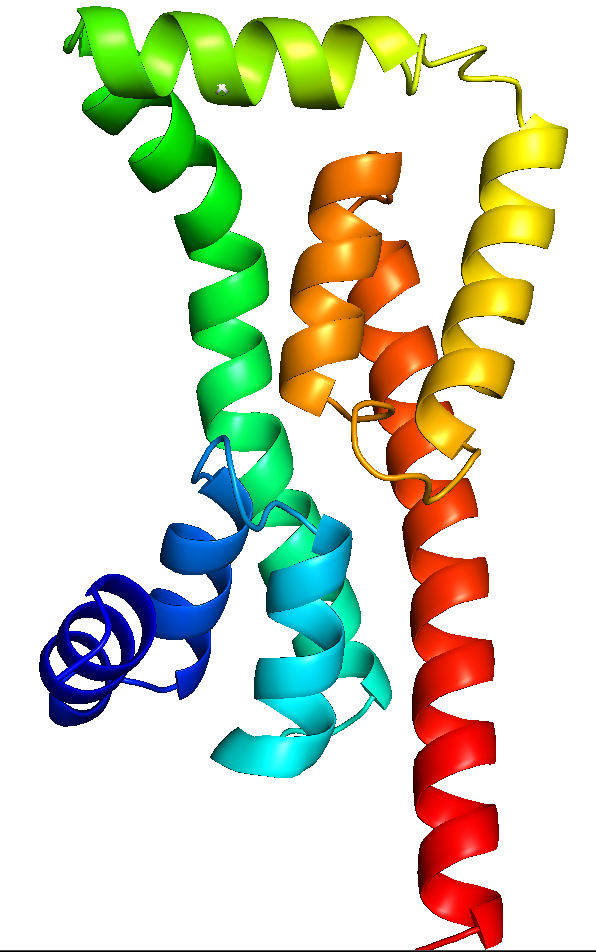
\includegraphics[width=\linewidth]{Results/w9_af.png}
  \caption{AF2 Mt2055 model}
  \label{fig:w9_af}
\end{subfigure}\hfil % <-- added
\caption{AlphaFold2 Modelling}
\small
Rainbow spectrum: N-terminal blue to C-terminal red.
\label{fig:af2_modelling}
\end{figure}


AF2 also gave rise to the opportunity to make structural predictions for another prominent member of the PF09335 family; Vmp1.  Attempts to model Vmp1 with Rosetta methods did not result in sensible models, even the DedA domain could not be modeled within the context of Vmp1.  Vmp1 is a 406 residue protein and Tmem41b forms complexes \emph{in vitro} and \emph{in vivo} with this other possible Atg protein \cite{Mizushima2011}. Molecular interaction of
Tmem41b is not detected with other Atg proteins. Tmem41b knockout cells exhibit inhibition of autophagosome formation and accumulation of lipid droplets \cite{Moretti2018} \cite{morita2018genome} Phenotypically Vmp1 knockout cells (KO) resemble Tmem41b KO cells indicating functional redundancy. Exogenous expression of the respective protein in the knockout cells restores function and the overexpression of Vmp1 in Tmem41b knockout cells restores autophagic flux with the reverse not being true \cite{Moretti2018}.

Examination of the Respre predicted contact map for Vmp1 (figure \ref{fig:vmp1}) predicts there is a bundle of three transmembrane helices on both the N-erminal and C-terminal sides of the conserved DedA structural domain.  Analysing the contact features of the DedA domain indicates an atypical pattern when comparing the equivalent region of the contact maps to other PF09335 homologues; the internal symmetry is broken. In the case of the C-terminal side of the DedA domains of Vmp1 the contact map can be interpreted in line with other PF09335 homologues displaying the common features as expected. However, the contact map features for the N-terminal symmetric half show a thirty-residue insertion between the first re-entrant loop and the proceeding transmembrane helix.  Here it can be seen that the TM helix simultaneously makes contact with the insertion and the C-terminal half of the re-entrant loop.  The insertion is highly conserved; this can be seen by the Consurf conservation mapping on the diagonal of the Vmp1 contact map.  The existence of this insertion could explain why Vmp1 is able carry out its function in the absence of Tmem41b while the reverse is not possible; the insertion may be a structurally essential feature not present in Tmem41b. The experimental evidence suggests that Vmp1 and Tmem41b oligomerise. It is possible that both homo-oligomers and hetero-oligomers form but only those where Vmp1 is present result in a functional protein.  

\begin{figure}[th!]
    \centering
    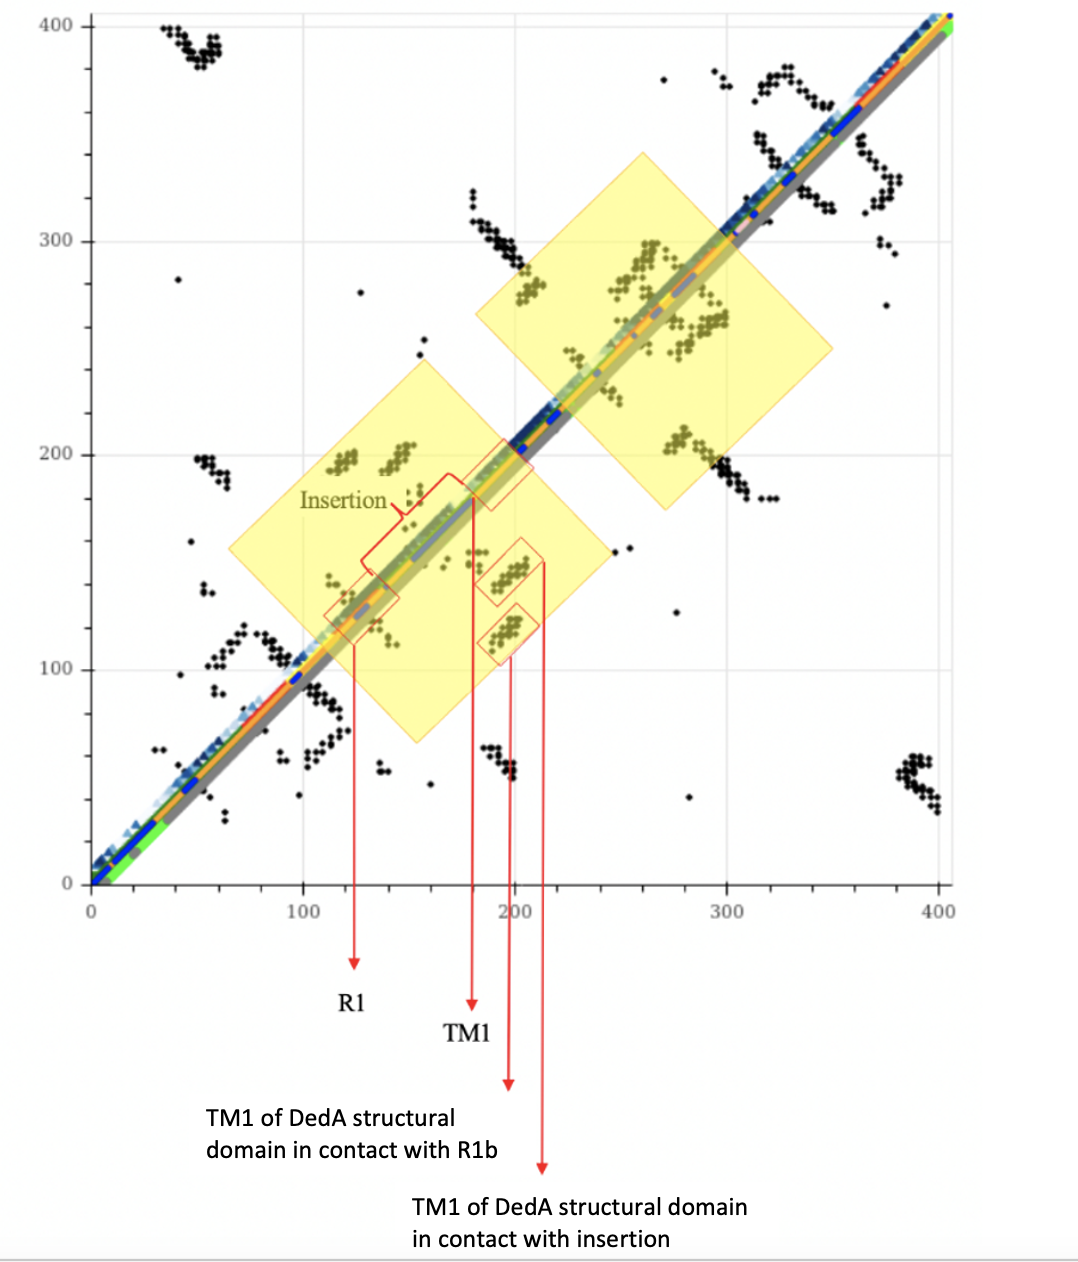
\includegraphics[width=150mm, scale =0.5]{Results/vmp1.png}
    \caption{Enhanced contact map for Vmp1}
    \label{fig:vmp1}
    \small
    Vmp-1 contact map constructed using DeepMetaPSICOV with additional information overlaid on the
diagonal. The outer diagonals show the TOPCONS membrane prediction (red regions being predicted TM helices, green; inside cell, yellow; outside). The thin central diagonal is the secondary structure prediction (orange, helix; blue, coil). Additionally, there is a blue spectrum diagonal which indicates levels of conservation from Consurf \cite{Ashkenazy2016} (the darker the blue the higher the level of conservation). Also, the grey (ordered) and lime green (disordered) diagonal utilises disorder predictions from IUPRED2a \cite{Meszaros2018}. R1 is the N-terminal re-entrant loop; R1b is the C-terminal half of the N-terminal re-entrant loop.
\end{figure}

Modelling of Vmp1 using AF2 produced a  model where most regions have a high pLDDT scores (Figure \ref{fig:vmp1_af}).  The model reveals three transmembrane helices upstream not in contact with each other and one downstream from the DedA domain.  This is in contrast to the predicted contact map where three transmembrane bundles are expected on both sides of the DedA domain. The familiar DedA domain features are clearly visible but with some differences.  Firstly, the N-terminal side amphipathic helix of the DedA domain is missing and an additional amphipathic helix is present on the C-terminal side of the DedA structural domain.  Secondly there is a loop region between the first re-entrant loop and the proceeding transmembrane helix, placing this region at the entrance of a putative channel.  The loop region corresponds to the insertion highlighted in the examination of the contact map, however, as opposed to the interpretation of the predicted contact map, in the AF2 model the loop insertion is not in contact with the proceeding transmembrane helix as the contact map suggested (Figure \ref{fig:vmp1_topt}). 


\begin{figure}[th!]
    \centering
    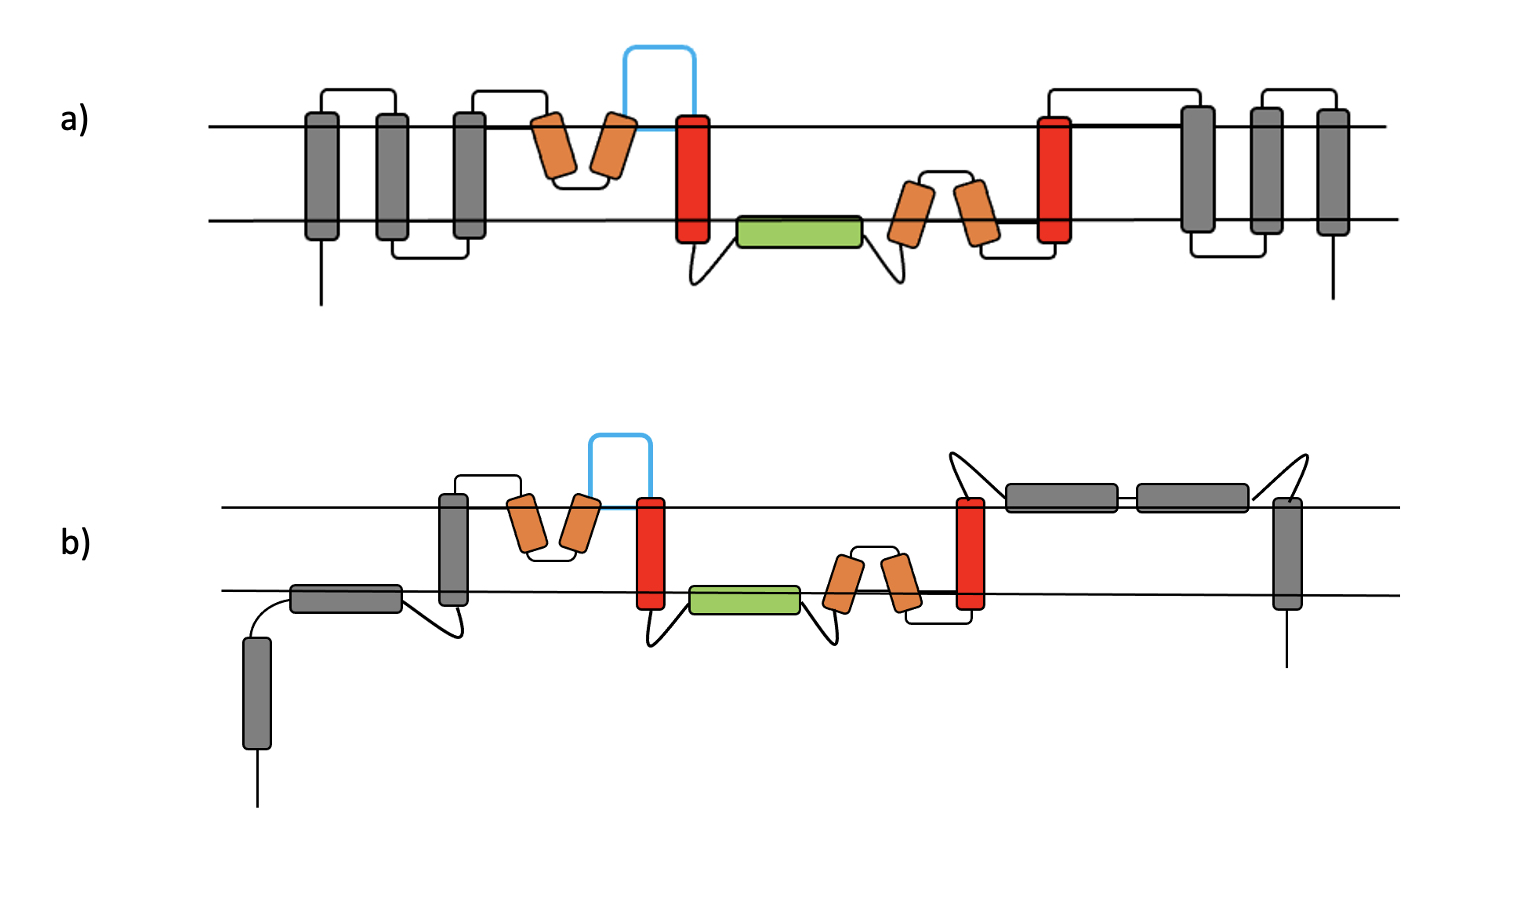
\includegraphics[width=170mm, scale =1]{Results/vmp1_topo.png}
    \caption{Topology of Vmp1 derived from the AF2 model}
    \label{fig:vmp1_topt}
    Grey: Helices that are additional to the established DedA core; red: TM helices belonging to the established DedA domain; orange; re-entrant loops belonging to the established DedA domain; green: amphipathic helices belonging to the established DedA domain; Blue: Highly conserved DedA domain loop insert.  a) Vmp predicted topology derived from predicted contact map analysis.  The presence of the amphipathic helix cannot be extrapolated from the predicted contact map, it's presence here is assumed based on helical secondary structure prediction and reference to the DedA domain topology to homologues.  The absence, compared other members of the DedA superfamily, of the N-terminal side amphipathic helix is assumed to to the lack of helix seconary structure allocation in this region.  b) Vmp predicted topology derived from predicted AF2 structure analysis.
    \small
    
\end{figure}


The discrepancy between the model and the interpretation of the ResPre predicted contact map can be explained by the fact that if the protein exists in multiple conformations, the contact map would be a superpostion of all the alternative conformations; the AF2 would be a representation of one of these conformations.  Additionally comparing predicated contact maps derived from alternative methods show that there is a lack of consistency between the various algorithms being used to generating co-variance data for Vmp1.

Further structural examination of the loop insertion modelled by AF2 was limited as unfortunately the local quality pLDDT scoring for this region is low.  ConSurf mapping of residue conservation for the insertion loop shows highly conserved regions along this structure. HHpred was used to query the PDB with the sequence making up the length of the mysterious loop, however, no hits were reported.

\begin{figure}[th!]
    \centering
    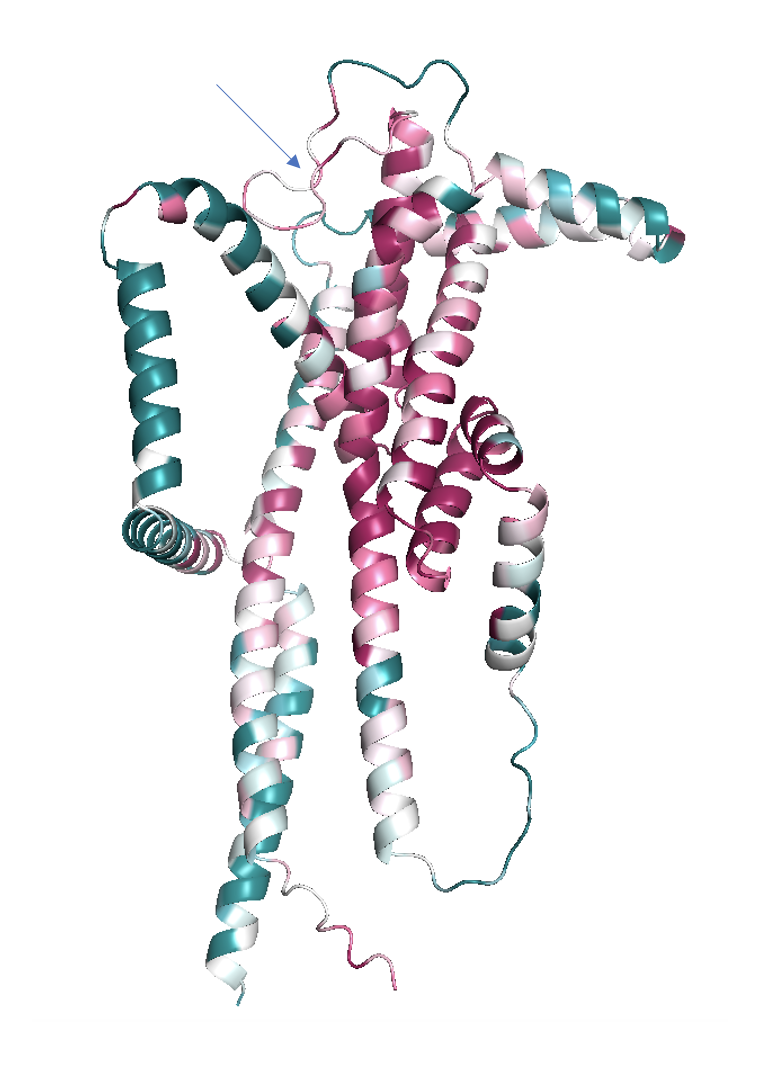
\includegraphics[width=100mm, scale =0.5]{Results/vmp1_af_consurf.png}
    \caption{Vmp1 AF2 model with ConSurf conservation mapping }
    \label{fig:vmp1_af}
    \small
    Arrow indication to conserved loop region.
\end{figure}

Examination of the N-terminal half contact map features of the AF2 Vmp1 model does show poor correlation with the predicted contact of the same region (Figure \ref{fig:vmp1_af_cmap}).  This indicates the N-terminal half may not be a valid structural prediction.  Vmp1 is part of the DedA family but with an atypical N-teminal domain.  AF2 uses the MSA to aid the modelling; any deep MSA will contain other members of the DedA family thereby maybe introducing noise into the N-terminal domain.  The introduction of this noise could impact on modelling in this region.  The introduction of noise through generation of deep MSAs built using a metagenomic database (during a separate piece of research - data not shown) has been shown result in contact signal loss and consequent decrease in model accuracy.

\begin{figure}[th!]
    \centering
    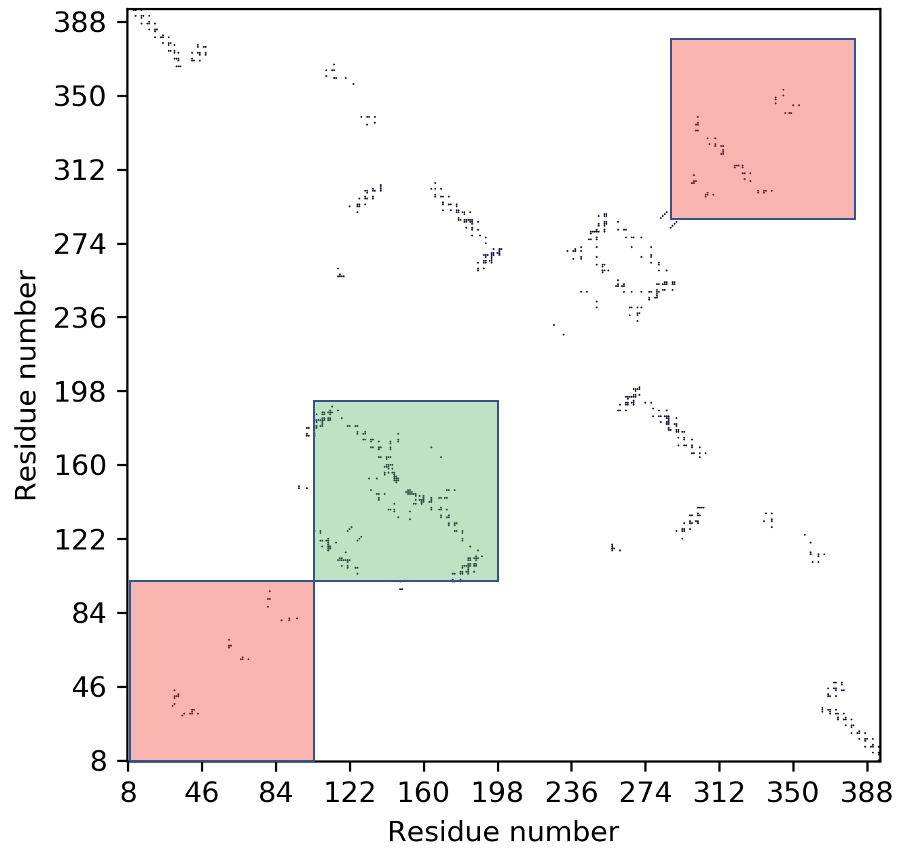
\includegraphics[width=100mm, scale =0.5]{Results/af_vmp1_cmap.png}
    \caption{Vmp1 AF2 model contact map}
    \label{fig:vmp1_af_cmap}
    \small
    Red boxes highlight missing three-helical bundles present on predicted contact map. Green box highlights N-terminal hald of DedA domain where the AF2 model contact features do not correlate with the predictions.
\end{figure}


\section{Potential homology between the DedA family and ABC transporters}
Performing a HHpred search with the Tmem41b sequence against the full PDB results in a strong hit against the Type I ABC transporter 3d31C. The hit has a 90\% probability and is across the whole length of the sequence.  This finding along with the ABC transporter structural hit with models where the re-entrant loop is forced into a transmembrane conformation points to the possibility that DedA proteins maybe related to ABC transporters.   A similar link has been suggested for the transmembrane autophagy protein Atg9 where the N- and C- terminal domains share membrane and tertiary topology (i.e. have a repeat) with sequence similarity identified locally around proline residues in the re-entrant loops and sequence similarity to N- terminal region of the transmembrane domains of T1 ABC exporters \cite{zhang2021evolution}.\\

A comparison of the proposed topology of Tmem41b with the topology of 3d31C (figure \ref{fig:abc_topology}) does indeed support an evolutionary link between the two where one side of the re-entrant loop has flipped forming a straight transmembrane helix or alternatively one half of the transmembrane helix has flipped forming a V-shaped re-entrant loop.  This 'flipping' has been shown previously in CPA/AT transporters \cite{sudha2021evolutionary}.

\begin{figure}[th!]
    \centering
    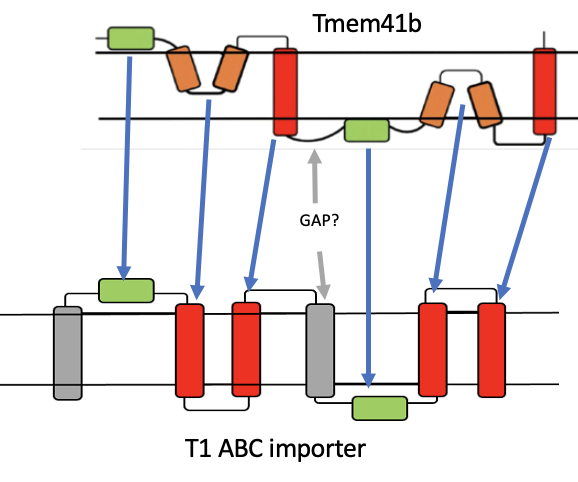
\includegraphics[width=100mm, scale =0.5]{Results/topology_comparison.png}
    \caption{Comparison of topologies of Tmem41b and 3d31C}
    \label{fig:abc_topology}
    \small
\end{figure}

However, analysis of the HHpred alignment (figure \ref{fig:abc_aln}) does reveal that the structural features do not correspond with each other in sequence indicating that the HHpred hit was a chance hit.

\begin{figure}[th!]
    \centering
    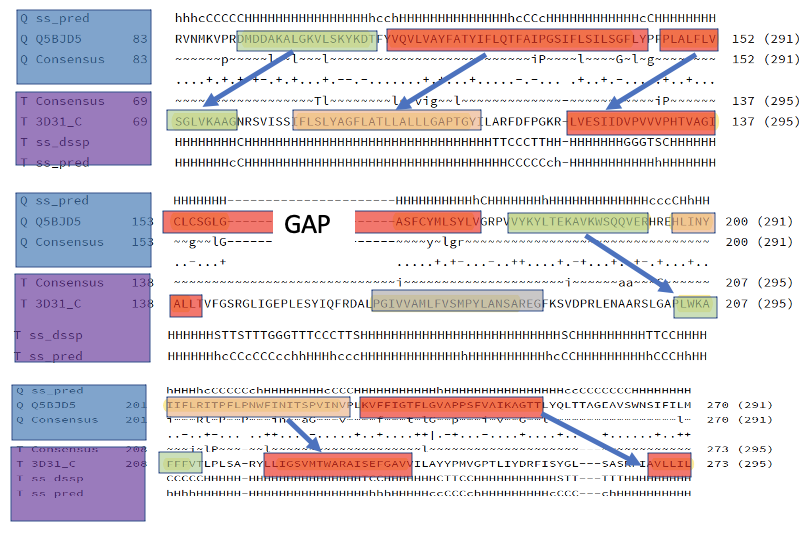
\includegraphics[width=100mm, scale =0.5]{Results/3d31c_aln.png}
    \caption{Annotated HHpred alignments of Tmem41b and 3d31C}
    \label{fig:abc_aln}
    \small
\end{figure}



\section{Conclusions}
Sequence, co-variance and ab initio modelling analyses show that the Pfam PF09335 and PF06695 domains are distantly homologous. These domains contain a structural core composed of a pseudo-inverse repeat of an amphipathic helix, a re-entrant loop and a TM helix. All PF09335 homologues contain this central core with additional TM- helices flanking either side.

Since the publication of this material \cite{mesdaghi2020silico}, the predictions made during this investigation in regard to the presence of re-entrant loops have been experimentally verified by cysteine accessibility method (SCAM) analysis for both Tmem41b \cite{okawa2021evolution} and Yqja \cite{scarsbrook2021topological}.  The presence of re-entrant loops in a transmembrane protein strongly indicates a transporter or pore functionality since this structural feature has, hitherto, only been found in proteins of this kind \cite{Yan2010} . The structural similarities between the DedA proteins and the Cl\textsuperscript{-}/H\textsuperscript{+} antiporters raise the possibility that the families studied here are, in fact, unsuspected distant homologues having several structural features in common. In that regard it is relevant to recall a hypothesis that DedA proteins are H\textsuperscript{+} antiporters as concluded from site-directed mutagenesis (SDM) experiments \cite{Kumar2014} \cite{Kumar2016}.

Querying the models against the PDB using DALI did not yield any significant hits. However, analysis of the prediction data revealed two features of DedA proteins that independently suggest that they are secondary transporters: both an inverted repeat architecture and the presence of a re-entrant loop, which are both independently and strongly associated with transporter function \cite{Duran2013} \cite{Yan2010}. Additionally, the fact that DedA proteins show structural similarities with H\textsuperscript{+} antiporters indicate that these proteins may also couple substrate transport with an opposing H\textsuperscript{+} current. Indeed, the YqjA homologue also contains strategically placed residues known to be involved in H\textsuperscript{+} antiporter activity. The ab initio models show that the essential residues come together in the region that would be buried in the membrane potentially forming a substrate chamber consistent with the transport of a specific substrate. Further research needs to be carried out to determine what this substrate is and confirm the mechanism of transport.

The investigation into Tmem41b demonstrates how covariance prediction data have multiple roles in modern structural bioinformatics: not just by acting as restraints for model making and serving for validation of the final models but by predicting domain boundaries and revealing the presence of cryptic internal repeats not evidenced by sequence analysis. Furthermore, contact map features were characterised and proven to be a re-entrant helix signal.  This ability to characterise contact map features in relation to re-entrant loops, was very exciting at the time as it gave the possibility to allow detection of this feature in other protein families by contact map analysis.  However, the acceleration in the advancement of ab initio modelling techniques such as AF2 has to some extent superseded the idea of using contact map features to predict the presence of structural features in uncharacterised proteins from contact maps; AF2 model databases can now be mined with query structures using methods like DALI, making the search for the contact map features obsolete.






